\documentclass{article}
\usepackage{iclr2027_conference,times}
%%%%% NEW MATH DEFINITIONS %%%%%

\usepackage{amsmath,amsfonts,bm}

% Mark sections of captions for referring to divisions of figures
\newcommand{\figleft}{{\em (Left)}}
\newcommand{\figcenter}{{\em (Center)}}
\newcommand{\figright}{{\em (Right)}}
\newcommand{\figtop}{{\em (Top)}}
\newcommand{\figbottom}{{\em (Bottom)}}
\newcommand{\captiona}{{\em (a)}}
\newcommand{\captionb}{{\em (b)}}
\newcommand{\captionc}{{\em (c)}}
\newcommand{\captiond}{{\em (d)}}

% Highlight a newly defined term
\newcommand{\newterm}[1]{{\bf #1}}


% Figure reference, lower-case.
\def\figref#1{figure~\ref{#1}}
% Figure reference, capital. For start of sentence
\def\Figref#1{Figure~\ref{#1}}
\def\twofigref#1#2{figures \ref{#1} and \ref{#2}}
\def\quadfigref#1#2#3#4{figures \ref{#1}, \ref{#2}, \ref{#3} and \ref{#4}}
% Section reference, lower-case.
\def\secref#1{section~\ref{#1}}
% Section reference, capital.
\def\Secref#1{Section~\ref{#1}}
% Reference to two sections.
\def\twosecrefs#1#2{sections \ref{#1} and \ref{#2}}
% Reference to three sections.
\def\secrefs#1#2#3{sections \ref{#1}, \ref{#2} and \ref{#3}}
% Reference to an equation, lower-case.
\def\eqref#1{equation~\ref{#1}}
% Reference to an equation, upper case
\def\Eqref#1{Equation~\ref{#1}}
% A raw reference to an equation---avoid using if possible
\def\plaineqref#1{\ref{#1}}
% Reference to a chapter, lower-case.
\def\chapref#1{chapter~\ref{#1}}
% Reference to an equation, upper case.
\def\Chapref#1{Chapter~\ref{#1}}
% Reference to a range of chapters
\def\rangechapref#1#2{chapters\ref{#1}--\ref{#2}}
% Reference to an algorithm, lower-case.
\def\algref#1{algorithm~\ref{#1}}
% Reference to an algorithm, upper case.
\def\Algref#1{Algorithm~\ref{#1}}
\def\twoalgref#1#2{algorithms \ref{#1} and \ref{#2}}
\def\Twoalgref#1#2{Algorithms \ref{#1} and \ref{#2}}
% Reference to a part, lower case
\def\partref#1{part~\ref{#1}}
% Reference to a part, upper case
\def\Partref#1{Part~\ref{#1}}
\def\twopartref#1#2{parts \ref{#1} and \ref{#2}}

\def\ceil#1{\lceil #1 \rceil}
\def\floor#1{\lfloor #1 \rfloor}
\def\1{\bm{1}}
\newcommand{\train}{\mathcal{D}}
\newcommand{\valid}{\mathcal{D_{\mathrm{valid}}}}
\newcommand{\test}{\mathcal{D_{\mathrm{test}}}}

\def\eps{{\epsilon}}


% Random variables
\def\reta{{\textnormal{$\eta$}}}
\def\ra{{\textnormal{a}}}
\def\rb{{\textnormal{b}}}
\def\rc{{\textnormal{c}}}
\def\rd{{\textnormal{d}}}
\def\re{{\textnormal{e}}}
\def\rf{{\textnormal{f}}}
\def\rg{{\textnormal{g}}}
\def\rh{{\textnormal{h}}}
\def\ri{{\textnormal{i}}}
\def\rj{{\textnormal{j}}}
\def\rk{{\textnormal{k}}}
\def\rl{{\textnormal{l}}}
% rm is already a command, just don't name any random variables m
\def\rn{{\textnormal{n}}}
\def\ro{{\textnormal{o}}}
\def\rp{{\textnormal{p}}}
\def\rq{{\textnormal{q}}}
\def\rr{{\textnormal{r}}}
\def\rs{{\textnormal{s}}}
\def\rt{{\textnormal{t}}}
\def\ru{{\textnormal{u}}}
\def\rv{{\textnormal{v}}}
\def\rw{{\textnormal{w}}}
\def\rx{{\textnormal{x}}}
\def\ry{{\textnormal{y}}}
\def\rz{{\textnormal{z}}}

% Random vectors
\def\rvepsilon{{\mathbf{\epsilon}}}
\def\rvtheta{{\mathbf{\theta}}}
\def\rva{{\mathbf{a}}}
\def\rvb{{\mathbf{b}}}
\def\rvc{{\mathbf{c}}}
\def\rvd{{\mathbf{d}}}
\def\rve{{\mathbf{e}}}
\def\rvf{{\mathbf{f}}}
\def\rvg{{\mathbf{g}}}
\def\rvh{{\mathbf{h}}}
\def\rvu{{\mathbf{i}}}
\def\rvj{{\mathbf{j}}}
\def\rvk{{\mathbf{k}}}
\def\rvl{{\mathbf{l}}}
\def\rvm{{\mathbf{m}}}
\def\rvn{{\mathbf{n}}}
\def\rvo{{\mathbf{o}}}
\def\rvp{{\mathbf{p}}}
\def\rvq{{\mathbf{q}}}
\def\rvr{{\mathbf{r}}}
\def\rvs{{\mathbf{s}}}
\def\rvt{{\mathbf{t}}}
\def\rvu{{\mathbf{u}}}
\def\rvv{{\mathbf{v}}}
\def\rvw{{\mathbf{w}}}
\def\rvx{{\mathbf{x}}}
\def\rvy{{\mathbf{y}}}
\def\rvz{{\mathbf{z}}}

% Elements of random vectors
\def\erva{{\textnormal{a}}}
\def\ervb{{\textnormal{b}}}
\def\ervc{{\textnormal{c}}}
\def\ervd{{\textnormal{d}}}
\def\erve{{\textnormal{e}}}
\def\ervf{{\textnormal{f}}}
\def\ervg{{\textnormal{g}}}
\def\ervh{{\textnormal{h}}}
\def\ervi{{\textnormal{i}}}
\def\ervj{{\textnormal{j}}}
\def\ervk{{\textnormal{k}}}
\def\ervl{{\textnormal{l}}}
\def\ervm{{\textnormal{m}}}
\def\ervn{{\textnormal{n}}}
\def\ervo{{\textnormal{o}}}
\def\ervp{{\textnormal{p}}}
\def\ervq{{\textnormal{q}}}
\def\ervr{{\textnormal{r}}}
\def\ervs{{\textnormal{s}}}
\def\ervt{{\textnormal{t}}}
\def\ervu{{\textnormal{u}}}
\def\ervv{{\textnormal{v}}}
\def\ervw{{\textnormal{w}}}
\def\ervx{{\textnormal{x}}}
\def\ervy{{\textnormal{y}}}
\def\ervz{{\textnormal{z}}}

% Random matrices
\def\rmA{{\mathbf{A}}}
\def\rmB{{\mathbf{B}}}
\def\rmC{{\mathbf{C}}}
\def\rmD{{\mathbf{D}}}
\def\rmE{{\mathbf{E}}}
\def\rmF{{\mathbf{F}}}
\def\rmG{{\mathbf{G}}}
\def\rmH{{\mathbf{H}}}
\def\rmI{{\mathbf{I}}}
\def\rmJ{{\mathbf{J}}}
\def\rmK{{\mathbf{K}}}
\def\rmL{{\mathbf{L}}}
\def\rmM{{\mathbf{M}}}
\def\rmN{{\mathbf{N}}}
\def\rmO{{\mathbf{O}}}
\def\rmP{{\mathbf{P}}}
\def\rmQ{{\mathbf{Q}}}
\def\rmR{{\mathbf{R}}}
\def\rmS{{\mathbf{S}}}
\def\rmT{{\mathbf{T}}}
\def\rmU{{\mathbf{U}}}
\def\rmV{{\mathbf{V}}}
\def\rmW{{\mathbf{W}}}
\def\rmX{{\mathbf{X}}}
\def\rmY{{\mathbf{Y}}}
\def\rmZ{{\mathbf{Z}}}

% Elements of random matrices
\def\ermA{{\textnormal{A}}}
\def\ermB{{\textnormal{B}}}
\def\ermC{{\textnormal{C}}}
\def\ermD{{\textnormal{D}}}
\def\ermE{{\textnormal{E}}}
\def\ermF{{\textnormal{F}}}
\def\ermG{{\textnormal{G}}}
\def\ermH{{\textnormal{H}}}
\def\ermI{{\textnormal{I}}}
\def\ermJ{{\textnormal{J}}}
\def\ermK{{\textnormal{K}}}
\def\ermL{{\textnormal{L}}}
\def\ermM{{\textnormal{M}}}
\def\ermN{{\textnormal{N}}}
\def\ermO{{\textnormal{O}}}
\def\ermP{{\textnormal{P}}}
\def\ermQ{{\textnormal{Q}}}
\def\ermR{{\textnormal{R}}}
\def\ermS{{\textnormal{S}}}
\def\ermT{{\textnormal{T}}}
\def\ermU{{\textnormal{U}}}
\def\ermV{{\textnormal{V}}}
\def\ermW{{\textnormal{W}}}
\def\ermX{{\textnormal{X}}}
\def\ermY{{\textnormal{Y}}}
\def\ermZ{{\textnormal{Z}}}

% Vectors
\def\vzero{{\bm{0}}}
\def\vone{{\bm{1}}}
\def\vmu{{\bm{\mu}}}
\def\vtheta{{\bm{\theta}}}
\def\va{{\bm{a}}}
\def\vb{{\bm{b}}}
\def\vc{{\bm{c}}}
\def\vd{{\bm{d}}}
\def\ve{{\bm{e}}}
\def\vf{{\bm{f}}}
\def\vg{{\bm{g}}}
\def\vh{{\bm{h}}}
\def\vi{{\bm{i}}}
\def\vj{{\bm{j}}}
\def\vk{{\bm{k}}}
\def\vl{{\bm{l}}}
\def\vm{{\bm{m}}}
\def\vn{{\bm{n}}}
\def\vo{{\bm{o}}}
\def\vp{{\bm{p}}}
\def\vq{{\bm{q}}}
\def\vr{{\bm{r}}}
\def\vs{{\bm{s}}}
\def\vt{{\bm{t}}}
\def\vu{{\bm{u}}}
\def\vv{{\bm{v}}}
\def\vw{{\bm{w}}}
\def\vx{{\bm{x}}}
\def\vy{{\bm{y}}}
\def\vz{{\bm{z}}}

% Elements of vectors
\def\evalpha{{\alpha}}
\def\evbeta{{\beta}}
\def\evepsilon{{\epsilon}}
\def\evlambda{{\lambda}}
\def\evomega{{\omega}}
\def\evmu{{\mu}}
\def\evpsi{{\psi}}
\def\evsigma{{\sigma}}
\def\evtheta{{\theta}}
\def\eva{{a}}
\def\evb{{b}}
\def\evc{{c}}
\def\evd{{d}}
\def\eve{{e}}
\def\evf{{f}}
\def\evg{{g}}
\def\evh{{h}}
\def\evi{{i}}
\def\evj{{j}}
\def\evk{{k}}
\def\evl{{l}}
\def\evm{{m}}
\def\evn{{n}}
\def\evo{{o}}
\def\evp{{p}}
\def\evq{{q}}
\def\evr{{r}}
\def\evs{{s}}
\def\evt{{t}}
\def\evu{{u}}
\def\evv{{v}}
\def\evw{{w}}
\def\evx{{x}}
\def\evy{{y}}
\def\evz{{z}}

% Matrix
\def\mA{{\bm{A}}}
\def\mB{{\bm{B}}}
\def\mC{{\bm{C}}}
\def\mD{{\bm{D}}}
\def\mE{{\bm{E}}}
\def\mF{{\bm{F}}}
\def\mG{{\bm{G}}}
\def\mH{{\bm{H}}}
\def\mI{{\bm{I}}}
\def\mJ{{\bm{J}}}
\def\mK{{\bm{K}}}
\def\mL{{\bm{L}}}
\def\mM{{\bm{M}}}
\def\mN{{\bm{N}}}
\def\mO{{\bm{O}}}
\def\mP{{\bm{P}}}
\def\mQ{{\bm{Q}}}
\def\mR{{\bm{R}}}
\def\mS{{\bm{S}}}
\def\mT{{\bm{T}}}
\def\mU{{\bm{U}}}
\def\mV{{\bm{V}}}
\def\mW{{\bm{W}}}
\def\mX{{\bm{X}}}
\def\mY{{\bm{Y}}}
\def\mZ{{\bm{Z}}}
\def\mBeta{{\bm{\beta}}}
\def\mPhi{{\bm{\Phi}}}
\def\mLambda{{\bm{\Lambda}}}
\def\mSigma{{\bm{\Sigma}}}

% Tensor
\DeclareMathAlphabet{\mathsfit}{\encodingdefault}{\sfdefault}{m}{sl}
\SetMathAlphabet{\mathsfit}{bold}{\encodingdefault}{\sfdefault}{bx}{n}
\newcommand{\tens}[1]{\bm{\mathsfit{#1}}}
\def\tA{{\tens{A}}}
\def\tB{{\tens{B}}}
\def\tC{{\tens{C}}}
\def\tD{{\tens{D}}}
\def\tE{{\tens{E}}}
\def\tF{{\tens{F}}}
\def\tG{{\tens{G}}}
\def\tH{{\tens{H}}}
\def\tI{{\tens{I}}}
\def\tJ{{\tens{J}}}
\def\tK{{\tens{K}}}
\def\tL{{\tens{L}}}
\def\tM{{\tens{M}}}
\def\tN{{\tens{N}}}
\def\tO{{\tens{O}}}
\def\tP{{\tens{P}}}
\def\tQ{{\tens{Q}}}
\def\tR{{\tens{R}}}
\def\tS{{\tens{S}}}
\def\tT{{\tens{T}}}
\def\tU{{\tens{U}}}
\def\tV{{\tens{V}}}
\def\tW{{\tens{W}}}
\def\tX{{\tens{X}}}
\def\tY{{\tens{Y}}}
\def\tZ{{\tens{Z}}}


% Graph
\def\gA{{\mathcal{A}}}
\def\gB{{\mathcal{B}}}
\def\gC{{\mathcal{C}}}
\def\gD{{\mathcal{D}}}
\def\gE{{\mathcal{E}}}
\def\gF{{\mathcal{F}}}
\def\gG{{\mathcal{G}}}
\def\gH{{\mathcal{H}}}
\def\gI{{\mathcal{I}}}
\def\gJ{{\mathcal{J}}}
\def\gK{{\mathcal{K}}}
\def\gL{{\mathcal{L}}}
\def\gM{{\mathcal{M}}}
\def\gN{{\mathcal{N}}}
\def\gO{{\mathcal{O}}}
\def\gP{{\mathcal{P}}}
\def\gQ{{\mathcal{Q}}}
\def\gR{{\mathcal{R}}}
\def\gS{{\mathcal{S}}}
\def\gT{{\mathcal{T}}}
\def\gU{{\mathcal{U}}}
\def\gV{{\mathcal{V}}}
\def\gW{{\mathcal{W}}}
\def\gX{{\mathcal{X}}}
\def\gY{{\mathcal{Y}}}
\def\gZ{{\mathcal{Z}}}

% Sets
\def\sA{{\mathbb{A}}}
\def\sB{{\mathbb{B}}}
\def\sC{{\mathbb{C}}}
\def\sD{{\mathbb{D}}}
% Don't use a set called E, because this would be the same as our symbol
% for expectation.
\def\sF{{\mathbb{F}}}
\def\sG{{\mathbb{G}}}
\def\sH{{\mathbb{H}}}
\def\sI{{\mathbb{I}}}
\def\sJ{{\mathbb{J}}}
\def\sK{{\mathbb{K}}}
\def\sL{{\mathbb{L}}}
\def\sM{{\mathbb{M}}}
\def\sN{{\mathbb{N}}}
\def\sO{{\mathbb{O}}}
\def\sP{{\mathbb{P}}}
\def\sQ{{\mathbb{Q}}}
\def\sR{{\mathbb{R}}}
\def\sS{{\mathbb{S}}}
\def\sT{{\mathbb{T}}}
\def\sU{{\mathbb{U}}}
\def\sV{{\mathbb{V}}}
\def\sW{{\mathbb{W}}}
\def\sX{{\mathbb{X}}}
\def\sY{{\mathbb{Y}}}
\def\sZ{{\mathbb{Z}}}

% Entries of a matrix
\def\emLambda{{\Lambda}}
\def\emA{{A}}
\def\emB{{B}}
\def\emC{{C}}
\def\emD{{D}}
\def\emE{{E}}
\def\emF{{F}}
\def\emG{{G}}
\def\emH{{H}}
\def\emI{{I}}
\def\emJ{{J}}
\def\emK{{K}}
\def\emL{{L}}
\def\emM{{M}}
\def\emN{{N}}
\def\emO{{O}}
\def\emP{{P}}
\def\emQ{{Q}}
\def\emR{{R}}
\def\emS{{S}}
\def\emT{{T}}
\def\emU{{U}}
\def\emV{{V}}
\def\emW{{W}}
\def\emX{{X}}
\def\emY{{Y}}
\def\emZ{{Z}}
\def\emSigma{{\Sigma}}

% entries of a tensor
% Same font as tensor, without \bm wrapper
\newcommand{\etens}[1]{\mathsfit{#1}}
\def\etLambda{{\etens{\Lambda}}}
\def\etA{{\etens{A}}}
\def\etB{{\etens{B}}}
\def\etC{{\etens{C}}}
\def\etD{{\etens{D}}}
\def\etE{{\etens{E}}}
\def\etF{{\etens{F}}}
\def\etG{{\etens{G}}}
\def\etH{{\etens{H}}}
\def\etI{{\etens{I}}}
\def\etJ{{\etens{J}}}
\def\etK{{\etens{K}}}
\def\etL{{\etens{L}}}
\def\etM{{\etens{M}}}
\def\etN{{\etens{N}}}
\def\etO{{\etens{O}}}
\def\etP{{\etens{P}}}
\def\etQ{{\etens{Q}}}
\def\etR{{\etens{R}}}
\def\etS{{\etens{S}}}
\def\etT{{\etens{T}}}
\def\etU{{\etens{U}}}
\def\etV{{\etens{V}}}
\def\etW{{\etens{W}}}
\def\etX{{\etens{X}}}
\def\etY{{\etens{Y}}}
\def\etZ{{\etens{Z}}}

% The true underlying data generating distribution
\newcommand{\pdata}{p_{\rm{data}}}
% The empirical distribution defined by the training set
\newcommand{\ptrain}{\hat{p}_{\rm{data}}}
\newcommand{\Ptrain}{\hat{P}_{\rm{data}}}
% The model distribution
\newcommand{\pmodel}{p_{\rm{model}}}
\newcommand{\Pmodel}{P_{\rm{model}}}
\newcommand{\ptildemodel}{\tilde{p}_{\rm{model}}}
% Stochastic autoencoder distributions
\newcommand{\pencode}{p_{\rm{encoder}}}
\newcommand{\pdecode}{p_{\rm{decoder}}}
\newcommand{\precons}{p_{\rm{reconstruct}}}

\newcommand{\laplace}{\mathrm{Laplace}} % Laplace distribution

\newcommand{\E}{\mathbb{E}}
\newcommand{\Ls}{\mathcal{L}}
\newcommand{\R}{\mathbb{R}}
\newcommand{\emp}{\tilde{p}}
\newcommand{\lr}{\alpha}
\newcommand{\reg}{\lambda}
\newcommand{\rect}{\mathrm{rectifier}}
\newcommand{\softmax}{\mathrm{softmax}}
\newcommand{\sigmoid}{\sigma}
\newcommand{\softplus}{\zeta}
\newcommand{\KL}{D_{\mathrm{KL}}}
\newcommand{\Var}{\mathrm{Var}}
\newcommand{\standarderror}{\mathrm{SE}}
\newcommand{\Cov}{\mathrm{Cov}}
% Wolfram Mathworld says $L^2$ is for function spaces and $\ell^2$ is for vectors
% But then they seem to use $L^2$ for vectors throughout the site, and so does
% wikipedia.
\newcommand{\normlzero}{L^0}
\newcommand{\normlone}{L^1}
\newcommand{\normltwo}{L^2}
\newcommand{\normlp}{L^p}
\newcommand{\normmax}{L^\infty}

\newcommand{\parents}{Pa} % See usage in notation.tex. Chosen to match Daphne's book.

\DeclareMathOperator*{\argmax}{arg\,max}
\DeclareMathOperator*{\argmin}{arg\,min}

\DeclareMathOperator{\sign}{sign}
\DeclareMathOperator{\Tr}{Tr}
\let\ab\allowbreak


\usepackage[utf8]{inputenc}
\usepackage[T1]{fontenc}
\usepackage{hyperref}
\usepackage{url}
\usepackage{booktabs}
\usepackage{amsfonts}
\usepackage{nicefrac}
\usepackage{microtype}
\usepackage{xcolor}
\usepackage{tabularx}
\usepackage{times}
\usepackage{soul}
\usepackage{caption}
\usepackage{graphicx}
\usepackage{subcaption}
\usepackage{amsmath}
\usepackage{amsthm}
\usepackage{amssymb}
\usepackage{algorithm}
\usepackage{algorithmicx}
\usepackage[noend]{algpseudocode}
\usepackage{multicol}
\usepackage{wrapfig}
\usepackage{multirow}
\usepackage{comment}
\usepackage{enumitem}
\usepackage{fancyvrb}
\usepackage{fvextra}
\usepackage{tikz}
\usetikzlibrary{positioning,shapes.geometric,shapes.misc,arrows.meta,fit,backgrounds}

\newtheorem{definition}{Definition}
\newtheorem{theorem}{Theorem}
\newtheorem{lemma}{Lemma}
\newtheorem{proposition}{Proposition}
\newtheorem{example}{Example}
\newtheorem{remark}{Remark}

\newcommand{\pr}[1]{\mathbb{P}\!\left( #1 \right)}
\newcommand{\coupling}[1]{\textsc{#1}}
\newcommand{\sense}[1]{\textsf{#1}}
\newcommand{\LCS}{\mathrm{LCS}}
\newcommand{\readout}[1]{\ensuremath{\mathrm{#1}}}
\newcommand{\mm}{\readout{mm}}
\newcommand{\cons}{\readout{cn}}
\newcommand{\rei}{\readout{re}}
\newcommand{\lp}{\readout{lp}}
\newcommand{\ent}{\coupling{entailment}}
\newcommand{\con}{\coupling{contradiction}}
\newcommand{\eqv}{\coupling{equivalence}}
\newcommand{\exc}{\coupling{exclusive}}
\newcommand{\cnc}{\coupling{co\_necessity}}

% Verbatim style for the prompt appendix.
\DefineVerbatimEnvironment{promptverb}{Verbatim}%
  {fontsize=\scriptsize,frame=single,framesep=3pt,numbers=left,numbersep=3pt,
   breaklines=true,breakanywhere=true,commandchars=\\\{\}}
\newcommand{\promptfile}[1]{%
  \VerbatimInput[fontsize=\scriptsize,frame=single,framesep=3pt,numbers=left,
                 numbersep=3pt,breaklines=true,breakanywhere=true]{#1}}

\newcommand{\rung}[1]{\texttt{#1}}
\newcommand{\famtype}[1]{\textsc{#1}}
\newcommand{\gate}[1]{\textsf{#1}}
\algrenewcommand\algorithmicindent{0.6em}

%\iclrfinalcopy


% Placeholder for numbers that depend on the extended (50-family) corpus or on the human
% studies of Section~\ref{sec-human}. Every occurrence must be filled before submission;
% `grep -n tbd main.tex` lists them.
\newcommand{\tbd}[1]{\textcolor{red}{[#1]}}

\title{LoCoBench: A Benchmark of Coherence Ladders for\\
       Evaluating Logical Coherence Measures}

\author{Anonymous authors\\Paper under double-blind review}

\begin{document}
\maketitle

\begin{abstract}
Measuring whether a long-form response \emph{hangs together} --- whether the claims it asserts form a
consistent argument rather than a bag of individually checkable facts --- requires evaluation data that
no existing resource provides. Two documents that differ in coherence almost always differ in topic,
length and content too, so a score difference between them cannot be attributed to coherence; human
ratings supply a target but not a controlled contrast; and no resource supplies the \emph{relation
graph} that would let a measure's scoring errors be separated from its relation-extraction errors. We
introduce \textbf{LoCoBench}, built from \emph{coherence ladders}: families of five responses over one
claim set that differ in one controlled structural respect, whose relative ordering is declared before
any measurement, and whose every rung carries its own machine-readable gold relation graph. Four ladder
types vary conflict structure, entailment-chain integrity and assertion order, and include a control
whose rungs must all score \emph{identically}. Families are generated by a five-stage prompted pipeline
and admitted only after an independent cross-vendor committee, which excludes the generator, certifies
that the prose realizes its planned relations, reads as expert prose, and asserts every planned claim.
The corpus supplies gold data for six discourse senses --- including exhaustive alternatives and resolved
concessions --- that no existing dataset labels. On \tbd{50} families and \tbd{250} responses, a
probabilistic coherence measure scored from gold graphs satisfies \tbd{82.7\%} of declared constraints,
while the same measure scored from mined graphs satisfies \tbd{34.7--37.1\%} and fails every invariance
check, and the best relation extractor reaches \tbd{51.9\%} coupling-level F1: the bottleneck is relation
extraction, not scoring. A pilot human study finds that readers agree with the declared ordering on
$8/10$ increase comparisons ($\alpha=0.75$), and identifies one ladder type whose declared invariance
readers reject; we specify a four-part human validation protocol, release all prompts verbatim, and
release rejected families with their reasons.
\end{abstract}

%% ================================================================
\section{Introduction}
\label{sec-intro}
%% ================================================================

Long-form factuality evaluation decomposes a response into atomic claims and verifies each against
retrieved evidence \citep{factscore,safe,veriscore}. The paradigm cannot see whether the claims form an
argument. A response asserting both that no one was harmed in an incident and that three people died
contains one true claim and one false one, and per-claim verification reports exactly that, without
registering that the response contradicts itself; a chain of true statements joined by a spurious
``therefore'' has no unsupported atom in it at all. \citet{lorefact} quantify the omission: on
logic-related samples, SAFE, VeriScore and FactCheck-GPT miss the logical dimension on $60\%$, $78\%$
and $48\%$ of cases respectively.

Measures of \emph{logical coherence} that address this exist or can be built --- from entity grids
\citep{barzilay} and their neural successors \citep{li} through discourse-representation scores
\citep{discoscore} and reasoning-chain metrics \citep{roscoe} to LLM judges \citep{geval} and
probabilistic models over claim-relation graphs. What does not exist is the data to evaluate them on.
This paper builds it.

\paragraph{Why ordinary corpora will not do.} The natural experiment --- score a set of documents and
correlate against human coherence ratings --- has three compounding defects. \emph{Confounding}: two
documents that differ in coherence differ in topic, length, register and claim content as well, so a
measure that tracks length or claim count can correlate respectably with ratings for reasons unrelated to
coherence. \emph{No ground truth for the mechanism}: a rating says a document is incoherent, not
\emph{which claims} are in tension, so a measure that is right for the wrong reason is indistinguishable
from one that is right. \emph{No separation of error sources}: a measure that builds an explicit relation
graph both extracts relations and scores them, and a rating cannot say which of the two failed.

\paragraph{What LoCoBench provides instead.} We build families of responses --- \emph{ladders} --- over
a single claim set, where the rungs differ only in a controlled structural respect and their relative
ordering is \emph{declared before any measurement}. A conflict ladder, for example, holds topic, claims and
every unperturbed relation fixed while varying only the conflict structure. Because the rungs share a
claim set, satisfying the declared ordering is attributable to coherence and not to content; and because
two ladder types declare that every rung must score \emph{identically}, the benchmark can catch a measure
that tracks the fact of having been edited rather than coherence. Every rung ships with a gold relation
graph --- which claims are related, by which discourse sense, in which direction, at what strength, and
whether the relation genuinely holds or is a planted error --- so a measure can be run once on its own
extracted relations and once on the gold graph, and the difference is the extractor's contribution,
isolated by construction.

\paragraph{A documented gap in existing annotation.} Six of the twelve discourse senses in our scheme ---
\sense{Instantiation}, \sense{Restatement}, \sense{Contrast}, \sense{Concession}, \sense{Alternative} and
\sense{Disjunction} --- have no gold data in any existing dataset we are aware of. Two of them are what
adjudicative prose turns on: an \sense{Alternative} is a pair of \emph{exhaustive} competing claims of which
exactly one holds, and a \sense{Concession} is a tension the text itself resolves. A measure that conflates
mere opposition with exhaustive opposition mis-scores every incident investigation and contested
judgement, and it cannot be caught doing so without labelled examples of both. Supplying them is a primary
purpose of the corpus.

\paragraph{Contributions.} We make four contributions, each stated with the evidence offered for it.

\begin{enumerate}[leftmargin=1.6em,itemsep=2pt,topsep=3pt]
\item \textbf{Coherence ladders as an evaluation design} (\S\ref{sec-scheme}--\S\ref{sec-ladders}). A
  formal definition of a ladder; a two-level annotation scheme whose discourse senses compile
  deterministically to truth-functional couplings; four ladder types that vary conflict structure,
  entailment-chain integrity and assertion order; and three classes of declared ordering constraint,
  including predicted inversions and exact invariances, which let the benchmark detect a measure that
  counts edits rather than measuring coherence.
\item \textbf{The LoCoBench corpus} (\S\ref{sec-corpus}--\S\ref{sec-schema}). \tbd{50} families and
  \tbd{250} responses over \tbd{36} topics in four domains, with per-rung gold relation graphs, planted
  invalid relations, declared non-relations as a genuine negative set, and gold data for six discourse
  senses no existing dataset labels.
\item \textbf{A reproducible generation and committee-validation pipeline}
  (\S\ref{sec-generation}--\S\ref{sec-validation}, Appendix~\ref{app-prompts}). Five prompted generation
  stages, ten perturbation calls with declared effects on the gold graph, and three validators run by a
  cross-vendor committee that excludes the generator. Every acceptance threshold is in one table, every
  prompt --- generation, validation, retry feedback, relation mining and judge baselines --- is reproduced
  verbatim and checked against the code by a test, and rejected families are released with their reasons.
\item \textbf{Validation of the benchmark, by measurement and by people} (\S\ref{sec-experiments}--%
  \S\ref{sec-human}). Evidence that the ladders discriminate between relation extractors and between
  coherence measures; a localization of current measures' failures in relation extraction rather than in
  scoring; a pilot human study; and a pre-registered four-study human validation protocol testing label
  validity, edit fidelity, perceived ordering, and committee--human agreement.
\end{enumerate}

%% ================================================================
\section{Related work}
\label{sec-related}
%% ================================================================

\paragraph{Factuality benchmarks and their blind spot.} FActScore \citep{factscore} pairs biography
prompts with a knowledge source and scores per-atom precision; SAFE \citep{safe} contributes
LongFact-Objects and search-augmented verification; VeriScore \citep{veriscore} restricts to verifiable
claims. Each supplies claims and evidence, and none supplies inter-claim structure, so none can serve as
evaluation data for a coherence measure. \citet{lorefact} is the closest prior art; it constructs data for
\emph{logic-related} fact-checking and labels dependencies between claims, but as a classification target
rather than as a graded ordering over controlled variants.

\paragraph{Perturbation-based coherence evaluation.} Evaluating coherence models against synthetic
perturbations is long established: entity-grid work \citep{barzilay} discriminates a document from its
sentence permutations, and neural coherence models \citep{li} add insertion and replacement perturbations.
LoCoBench inherits the methodology and changes one thing: the perturbation is an operation on a
\emph{declared relation graph}, whose effect on the graph is computed and recorded per rung, rather than an
operation on text whose effect on coherence is assumed. The benchmark can therefore say not only that rung
$k{+}1$ should score above rung $k$ but which relation changed, and --- for meaning-preserving edits ---
that two rungs must score \emph{identically}. Shuffling alone cannot express that distinction; indeed our
pilot study (\S\ref{sec-human}) suggests that the classic shuffle test measures something other than
logical coherence.

\paragraph{Discourse annotation as precedent.} Our sense inventory is grounded in PDTB~3.0 \citep{pdtb}
and RST \citep{mann}. Both establish that discourse relations can be annotated from surface cues, which is
what makes the relation-recovery gate of \S\ref{sec-validation} a reasonable demand. PDTB annotates
naturally occurring text, where the distribution of relations is whatever the corpus happens to contain ---
which is why six of our senses lack gold data. A generated corpus can \emph{require} the rare relations,
and ours does.

\paragraph{LLM-generated benchmarks, LLM judges, and their validation.} Generating evaluation data with a
language model is now common, and its known risks are circularity (the generator's biases become ground
truth), leakage (artifacts revealing the construction), and unverifiable labels. We address these
structurally --- a committee that excludes the generator, a leakage validator, and a gate requiring an
independent model to \emph{recover} the planned relations from the prose --- and empirically, with human
studies (\S\ref{sec-human}) whose design follows standard practice for annotation reliability
\citep{krippendorff}, paired-comparison modelling \citep{bradleyterry}, and the statistical justification of
LLM annotators against human ones \citep{altannotator}.

%% ================================================================
\section{The annotation scheme}
\label{sec-scheme}
%% ================================================================

An item's gold annotation is a graph over its claims. Edge labels come from a two-level scheme: an
interpretable \emph{discourse sense} that an annotator can read off surface cues, and an inferential
\emph{coupling} that says what the relation asserts about the joint truth of its endpoints. A deterministic
map connects the two levels, and that map --- not the annotator and not the generator --- is the authority
on what a sense means.

\subsection{Level one: inferential couplings}

\begin{definition}[Inferential couplings]
\label{def-couplings}
A coupling $\tau$ is specified by the set $V(\tau)\subseteq\{0,1\}^2$ of joint truth assignments
$(a_s,a_t)$ of its source and target claims that it \emph{penalizes}:
\begin{center}\small
\begin{tabular}{@{}llcl@{}}
\toprule
Coupling & Reading & Directed & Penalized set $V(\tau)$ \\
\midrule
\ent            & $a_s \Rightarrow a_t$              & yes & $\{(1,0)\}$ \\
\con            & $a_s \Rightarrow \neg a_t$         & yes & $\{(1,1)\}$ \\
\eqv            & $a_s \Leftrightarrow a_t$          & no  & $\{(0,1),(1,0)\}$ \\
\exc            & exactly one of $a_s,a_t$ holds     & no  & $\{(0,0),(1,1)\}$ \\
\cnc            & at least one of $a_s,a_t$ holds    & no  & $\{(0,0)\}$ \\
\coupling{none} & no truth coupling                  & --- & $\varnothing$ \\
\bottomrule
\end{tabular}
\end{center}
The two couplings whose penalized set contains the both-true world, $\{\con,\exc\}$, are the
\emph{conflict} couplings.
\end{definition}

The distinction between \con{} and \exc{} is the one the scheme exists to draw. \con{} forbids only the
both-true world: two claims that cannot both hold but might both fail. \exc{} additionally forbids the
both-false world, which is what an exhaustive pair asserts. \cnc{} is the dual, forbidding only the
both-false world, which is what a disjunction asserts. A scheme offering only \con{} can express neither,
and a measure evaluated against such a scheme is untested on precisely the relations adjudicated disputes
turn on.

\subsection{Level two: discourse senses, and the compile map}

\begin{definition}[Compile map]
\label{def-compile}
The compile map $\mathcal{C}$ assigns to each discourse sense a coupling, a strength prior ($\bot$ meaning
``use the estimated value''), and the flags \emph{directed}, \emph{concession} and \emph{ordering-only}. It
is total and deterministic, and is given in Table~\ref{tab:compile}.
\end{definition}

\begin{table}[t]
\centering\small
\caption{The compile map $\mathcal{C}$ of Def.~\ref{def-compile}, with the number of gold edges of each
  sense in the current release. \emph{Ordering-only} senses record assertion order but carry \textbf{no
  truth coupling}, so they produce no factor in any scorer that consumes the scheme. \textbf{Bold} marks the
  six senses for which we are aware of no gold data in any existing dataset. Counts are over all rungs of
  the \tbd{14}-family release; the \tbd{50}-family counts replace them.}
\label{tab:compile}
\begin{tabular}{@{}llccllr@{}}
\toprule
Level-2 sense & $\mathcal{C}$ coupling & prior & dir. & flag & gloss & edges \\
\midrule
\sense{Cause-Effect}   & \ent & $\bot$ & yes & & source brings target about & 69 \\
\sense{Effect-Cause}   & \ent & $\bot$ & yes & & source is the effect, target the cause & 5 \\
\sense{Evidence}       & \ent & $\bot$ & yes & & source is evidence for target & 82 \\
\sense{Condition}      & \ent & $\bot$ & yes & & source conditions target & 4 \\
\textbf{\sense{Instantiation}} & \ent & $\bot$ & yes & & target instantiates source & 38 \\
\textbf{\sense{Restatement}} & \eqv & $0.90$ & no & & definitional identity & 93 \\
\textbf{\sense{Contrast}}    & \con & $\bot$ & no & & opposed, \emph{not} exhaustive & 90 \\
\textbf{\sense{Concession}}  & \con & $\bot$ & yes & conc. & a tension the text resolves & 74 \\
\textbf{\sense{Alternative}} & \exc & $\bot$ & no & & exhaustive: exactly one holds & 78 \\
\textbf{\sense{Disjunction}} & \cnc & $\bot$ & no & & at least one holds & 70 \\
\sense{Precedence}     & \coupling{none} & --- & yes & ord. & temporal order only & 52 \\
\sense{Succession}     & \coupling{none} & --- & yes & ord. & temporal order only & 15 \\
\midrule
\multicolumn{6}{@{}l}{Total} & 670 \\
\bottomrule
\end{tabular}
\end{table}

Five senses collapse onto \ent{}, a deliberate loss of information at the inferential level: whether one
claim causes another or merely evidences it makes no difference to what the pair asserts about joint truth.
The sense is retained alongside the coupling so that error analysis can distinguish ``related, but
mislabelled'' from ``not related'', and so that the corpus serves work on the discourse layer for its own
sake.

\paragraph{The compile map is enforced.} A gold relation carries both a sense and a coupling, which
invites inconsistency. The schema validator rejects any item in which
$\text{coupling}\neq\mathcal{C}(\text{sense})$, and re-derives directedness, ordering-only status and
exhaustiveness from the sense rather than trusting the generator's assertion of them. This matters for a
generated corpus: an LLM asked for both a sense and a coupling will occasionally emit a pair no reading of
the scheme licenses, and keeping such an edge would place a factor in the graph that its sense does not
justify. Every gold edge in the corpus therefore uses one of the twelve $(\text{sense},\text{coupling})$
combinations of Table~\ref{tab:compile}.

%% ================================================================
\section{Coherence ladders}
\label{sec-ladders}
%% ================================================================

\begin{definition}[Coherence ladder]
\label{def-ladder}
A \emph{ladder} is a tuple $(\mathcal{P},\langle\rho_0,\dots,\rho_4\rangle,\Gamma)$ where $\mathcal{P}$ is
a base \emph{relation plan} --- a selected claim set with a declared relation graph over it --- each rung
$\rho_k$ is a sequence of perturbation operator calls applied to $\mathcal{P}$, yielding a response text
together with its \emph{own} gold relation graph, and $\Gamma$ is a set of constraints on the relative
ordering of the rungs' scores. A ladder is \emph{admitted} only as a whole (\S\ref{sec-validation}).
\end{definition}

\paragraph{Whole-family admission.} A ladder is admitted entire or not at all. Four of the five rungs carry
no standalone claim, only a claim relative to their neighbours, so a ladder missing a rung is not a partial
success but a broken comparison. Every gate therefore rejects at family granularity.

\begin{table}[t]
\centering\small
\caption{The four ladder types. Each holds the claim set, the topic and every unperturbed relation fixed,
  varying one structural dimension. Counts are the generator's proportional allocation at the release size
  of \tbd{50} families; the current release has $8/2/3/1$. The \famtype{order} and \famtype{control}
  patterns are declared with respect to \emph{logical} coherence: their edits change no truth coupling, so
  the gold graph, and any score computed from it, must not move. Whether \emph{readers} agree is an
  empirical question that the pilot study answers differently for the two types (\S\ref{sec-human}).}
\label{tab:ladders}
\begin{tabular}{@{}lp{2.3cm}p{4.6cm}p{2.7cm}r@{}}
\toprule
Type & Dimension varied & Rungs, $\rho_0 \to \rho_4$ & Declared pattern & $n$ \\
\midrule
\famtype{conflict} & conflict structure
  & \rung{worse}, \rung{base}, \rung{concession\_resolved}, \rung{fix\_one\_conflict}, \rung{coherent}
  & increasing, with one predicted dip & \tbd{24} \\[3pt]
\famtype{chain} & entailment-chain integrity
  & \rung{break\_3}, \rung{break\_2}, \rung{break\_1}, \rung{base}, \rung{coherent}
  & strictly increasing & \tbd{10} \\[3pt]
\famtype{order} & assertion order
  & \rung{shuffle\_full}, \rung{shuffle\_block}, \rung{shuffle\_adjacent}, \rung{base},
    \rung{ordering\_only}
  & \textbf{flat throughout} & \tbd{10} \\[3pt]
\famtype{control} & nothing (meaning-preserving)
  & \rung{ordering\_only}, \rung{direction\_reversal}, \rung{base}, \rung{direction\_reversal},
    \rung{ordering\_only}
  & \textbf{flat throughout} & \tbd{6} \\
\bottomrule
\end{tabular}
\end{table}

Table~\ref{tab:ladders} gives the four types. \famtype{conflict} is the reference ladder: only the conflict
structure varies. A spurious relation makes the lowest rung worse than the base; the upper rungs resolve
the conceded tension and then drop one and two conflict edges. \famtype{chain} breaks $N$ links of an
entailment chain, so the defect is a \emph{missing} relation rather than a present conflict --- a
distinction that matters because a measure built on contradiction detection alone will do well on the
first ladder and fail the second.

\famtype{order} and \famtype{control} are \emph{invariance} ladders. \famtype{order} permutes sentences at
three granularities and then exchanges a \sense{Precedence} for a \sense{Succession}; \famtype{control}
exchanges \sense{Precedence} for \sense{Succession} or reverses the direction of a symmetric relation. None
of these edits changes a truth coupling, so the declared pattern is a flat line and a measure that trends
across either has demonstrated that it responds to \emph{having been edited}. The two types are kept
separate on purpose. \famtype{control} edits are meaning-preserving for any reader. \famtype{order} edits
preserve every claim and every coupling but can strand an anaphor or put evidence after the conclusion it
supports --- they preserve \emph{logical} coherence while degrading \emph{discourse} coherence. Keeping the
types apart lets the benchmark, and the human study, ask whether a measure (or a reader) can tell those two
properties apart.

\subsection{Ordering constraints}
\label{sec-constraints}

A family declares its constraints in three classes, each asserted per \emph{readout} of the measure under
test, so that a family can declare that one readout must increase between two rungs while another is
unconstrained there.

\textbf{C1, strict increase.} Consecutive rungs must be strictly ordered.

\textbf{C2, predicted inversion or invariance.} A score must \emph{decrease}, or must be \emph{exactly
invariant}. This is what distinguishes a declared-ordering benchmark from a monotonicity test. Some readouts
are expected to dip when a conceded tension is resolved, because softening a conflict raises the
probability of the very configuration the conflict forbids; asserting the dip turns a known peculiarity
into a falsifiable prediction. And a coupling-free edit \emph{must} be exactly flat: C2 then asserts an
equality, and a measure that moves at all has been caught reading surface form.

\textbf{C3, endpoint separation.} The extreme rungs must separate (or, on the invariance ladders, must not),
for all readouts. This is the robust headline claim, insensitive to the fine structure of intermediate
rungs.

For the three-readout measure of \S\ref{sec-harness}, a \famtype{conflict} family declares $14$
constraints ($9$ C1, $2$ C2, $3$ C3) and every other family $15$ ($12$ C1 or C2 over the four adjacent
pairs, $3$ C3). The current release declares $202$; all are achievable by construction, in that no family
carries a constraint its own gold graphs cannot satisfy. A single-score measure inherits only the
readout-independent content: five increase assertions per \famtype{conflict} or \famtype{chain} family (four
C1 pairs and the C3 endpoints) and five invariance assertions per \famtype{order} or \famtype{control} family.
A measure is scored on the fraction of declared constraints it satisfies.

%% ================================================================
\section{The generation pipeline}
\label{sec-generation}
%% ================================================================

Generation is a five-stage prompted pipeline followed by validation, and the stages are separated so that a
defect can be attributed to one of them and repaired there. Each stage's prompt is fixed, versioned, and
reproduced verbatim in Appendix~\ref{app-prompts}; the appendix files are written from the source by a
script, and a test fails if any of them differs from the prompt the code issues.
Algorithm~\ref{alg:pipeline} gives the procedure end to end and Figure~\ref{fig:pipeline} its shape.

\begin{figure}[t]
\centering
\resizebox{\textwidth}{!}{%
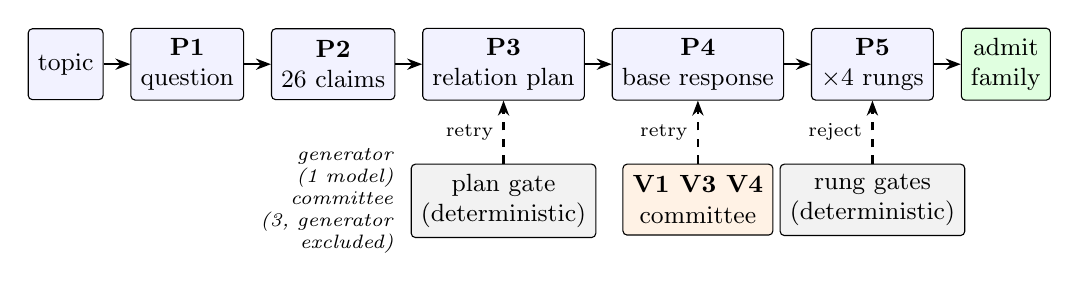
\begin{tikzpicture}[font=\small,
  st/.style={draw,rounded corners=1.5pt,align=center,inner sep=3.5pt,minimum height=9mm,fill=blue!5},
  vd/.style={draw,rounded corners=1.5pt,align=center,inner sep=3.5pt,minimum height=9mm,fill=orange!10},
  dt/.style={draw,rounded corners=1.5pt,align=center,inner sep=3.5pt,minimum height=9mm,fill=gray!10},
  fin/.style={draw,rounded corners=1.5pt,align=center,inner sep=3.5pt,minimum height=9mm,fill=green!12},
  ar/.style={-{Stealth[length=1.9mm]},thick}, node distance=3.4mm]
  \node[st] (t) {topic};
  \node[st,right=of t] (p1) {\textbf{P1}\\question};
  \node[st,right=of p1] (p2) {\textbf{P2}\\26 claims};
  \node[st,right=of p2] (p3) {\textbf{P3}\\relation plan};
  \node[st,right=of p3] (p4) {\textbf{P4}\\base response};
  \node[st,right=of p4] (p5) {\textbf{P5}\\$\times4$ rungs};
  \node[fin,right=of p5] (adm) {admit\\family};
  \foreach \a/\b in {t/p1,p1/p2,p2/p3,p3/p4,p4/p5,p5/adm} \draw[ar] (\a) -- (\b);
  \node[dt,below=8mm of p3] (g3) {plan gate\\(deterministic)};
  \node[vd,below=8mm of p4] (cv) {\textbf{V1 V3 V4}\\committee};
  \node[dt,below=8mm of p5] (g5) {rung gates\\(deterministic)};
  \draw[ar,dashed] (g3) -- node[left,font=\scriptsize]{retry} (p3);
  \draw[ar,dashed] (cv) -- node[left,font=\scriptsize]{retry} (p4);
  \draw[ar,dashed] (g5) -- node[left,font=\scriptsize]{reject} (p5);
  \node[left=1mm of g3,font=\scriptsize\itshape,align=right,text width=22mm]
    {generator (1 model)\\committee (3, generator\\excluded)};
\end{tikzpicture}}
\caption{The pipeline. Five generation stages produce a family of five rungs from one topic. The plan is
  checked by a deterministic gate, the base response by the three-model committee, and each perturbed rung
  by deterministic gates; gate failures are fed back to the generating stage as a retry, and a family that
  exhausts its retries is rejected whole and stored with its reason.}
\label{fig:pipeline}
\end{figure}

\begin{algorithm}[t]
\caption{Generating one family of type $T$ on topic $t$. \textsc{Ask}$(P,\cdot,g)$ calls prompt $P$, parses
  the output, applies check $g$, and on a parse or check failure re-issues the prompt with the failure
  reason appended (Appendix~\ref{app-retry}), up to $3$ attempts at temperatures $(\text{default},0.3,0.7)$.}
\label{alg:pipeline}
\begin{algorithmic}[1]
\State $q \gets \textsc{Ask}(\text{P1}, t)$ \Comment{open question}
\State $C \gets \textsc{Ask}(\text{P2}, q)$ \Comment{26 tagged claims}
\State $\mathcal{P} \gets \textsc{Ask}(\text{P3}, q, C,\ g{=}\textsc{PlanGate})$ \Comment{claims, 10 relations, non-relations}
\State $x_{\text{base}} \gets \textsc{Ask}(\text{P4}, q, \mathcal{P},\ g{=}\textsc{Committee})$ \Comment{V1, V3, V4}
\State $E_{\text{base}} \gets$ gold graph of $\mathcal{P}$, fields re-derived through $\mathcal{C}$
\State assign each operator call of each rung of $T$ a distinct eligible target edge; \textbf{reject} if too few
\For{each non-base rung $\rho_k$ of $T$, in ladder order}
  \For{each call $o$ of $\rho_k$}
    \State $x \gets \textsc{Ask}(\text{P5}, x, \mathcal{P}, o)$; \textbf{reject} unless $x$ changed and drift $\le 15\%$
  \EndFor
  \State $E_k \gets$ apply the declared edge effects of $\rho_k$'s calls to $E_{\text{base}}$
\EndFor
\State \textbf{reject} if two adjacent rungs have equal edge sets and the upper one claims a change
\State \textbf{reject} unless every item passes the schema validator; otherwise \textbf{admit} all five rungs
\end{algorithmic}
\end{algorithm}

\subsection{P1: topic to question}

Given a topic from the inventory of \S\ref{sec-corpus}, emit one open-ended question. Three of the nine
instructions do real work. The question must \emph{elicit} diverse logical structure, and the prompt
enumerates the target relations so that the question is chosen with the downstream plan in mind. It must
prefer adjudicative framings --- incident investigations, litigation, diagnostic reasoning, attribution
disputes, competing scientific hypotheses --- because these are where exhaustive alternatives and resolving
holdings arise naturally. And it must \emph{not} contain the words ``cause'', ``condition'',
``alternative'' or ``contrast'', so that the answer's relations are not primed lexically by the question.

\subsection{P2: question to tagged claims}

Emit exactly $26$ atomic claims, each a single declarative sentence with no connective joining it to
another --- relations are added at the next stage, so that the claim set and the relation graph are
independently controlled. The composition is specified: $14$ factually correct claims; $4$
plausible-but-false claims; an \emph{exhaustive alternative} pair, of which exactly one must be true; a
\emph{disjunctive} pair, of which at least one must be true; an \emph{equivalent} pair; and two
\emph{holding} claims in which an authority settles a dispute. Each claim carries a tag recording its role.
The disjunctive pair must be phrased as states of the world rather than as findings --- a pair of
\emph{reports} is trivially compatible and yields no real disjunction --- and the false claims must not be
signalled by hedging.

\subsection{P3: claims to relation plan}

The planning stage, and the most constrained. Select $14$--$16$ of the claims, renumber them to consecutive
assertion positions, and plan exactly ten relations over distinct claim pairs, each with a sense from
Table~\ref{tab:compile}, an intended strength band, and a \emph{validity} label. Five requirements shape the
output; a deterministic plan gate checks each, and a violation is fed back to the planner as a retry.

\emph{At least two false claims must be selected}, so the response asserts false content alongside true.
Without this quota the planner selected none, which would make coherence and factuality perfectly
correlated in the data. Two sits just below the expected $\approx 2.3$ under indifferent sampling of $15$
from $26$ claims with $4$ false.

\emph{Five senses are required} --- at least one \sense{Alternative}, \sense{Disjunction},
\sense{Restatement}, \sense{Concession} and temporal ordering --- and \emph{at least four of the ten
relations must carry a conflicting sense} (\sense{Alternative}, \sense{Concession} or \sense{Contrast}), at
most one of them a resolved \sense{Concession}. The first quota supplies the scarce senses; the second
guarantees the \famtype{conflict} ladder enough unresolved conflict edges to drop two of them and resolve a
third (\S\ref{sec-goldedges}). Without it, plans carried too few conflict edges and the ladder's upper rungs
could not be built.

\emph{Exactly six relations valid and four invalid}, each invalid relation carrying an error kind ---
\gate{wrong\_sense}, \gate{wrong\_direction}, \gate{false\_endpoint} or \gate{spurious}. Planted invalid
relations are asserted in the prose in the same register as valid ones, and make the corpus a test of
\emph{precision}: an extractor that recovers every gold edge including the planted ones has not exercised
judgement. The count is stated as a count because a planner asked for ``about $60\%$'' rounds unpredictably.

\emph{Four to six declared non-relations}: pairs of selected claims within four positions between which the
response must draw no dependence. Precision against all unlabelled pairs is close to meaningless, since most
are simply unannotated; a violated \emph{declared} non-relation is a genuine false positive against a real
negative set.

\emph{Relations are local by default}, preferring pairs within four positions, with long-range pairs
permitted when the two claims share a named entity --- a deliberate bias toward graphs a reader can recover,
so that a V1 failure indicates a defective realization rather than an unreasonable demand.

\subsection{P4: plan to response}

Write $550$--$650$ words of prose (floor $500$) realizing the plan exactly: assert every planned claim once,
in position order, and realize every planned relation so that a careful reader can recover it from the text
alone, while reading as publishable expert prose rather than as an annotation walked sentence by sentence.
Several instructions resolve that tension. Back-reference uses a pronoun or a noun phrase named after
\emph{the thing the claim is about}, not after its status as a finding. Quantifiers, numbers, dates,
polarity and modals are \emph{content}, so a claim may be reworded but not weakened. Exhaustive and
disjunctive pairs must make their logical strength \emph{explicit}, since a bare ``X, or Y'' leaves a reader
unable to tell \sense{Alternative} from \sense{Disjunction}. Temporal orderings must be stated within one
sentence. Non-relations are separated by distance and paragraphing rather than by an explicit marker, which
would both leak the plan and itself draw a relation. The prompt forbids mentioning the plan, its labels, or
the fact that some content is incorrect.

\subsection{P5: response to rung}

Apply exactly one perturbation to the current text, changing the minimum number of words and preserving
everything else verbatim; a rung composed of several calls applies them in sequence.
Table~\ref{tab:operators} gives the ten calls, grouped by the six operators they realize. Length drift is
capped at $15\%$, except for the three calls that add or remove a sentence by definition.

\begin{table}[t]
\centering\small
\caption{The six perturbation operators and the ten parameterized calls realizing them. Each call has a
  declared effect on the rung's gold relation graph (\S\ref{sec-goldedges}). The two \famtype{o6} calls and
  \gate{direction\_reversal} on a symmetric relation are coupling-invariant: they are what the
  \famtype{order} and \famtype{control} ladders exist to check.}
\label{tab:operators}
\begin{tabular}{@{}lp{3.3cm}p{6.6cm}@{}}
\toprule
Op & Calls & Effect on the text \\
\midrule
\famtype{o1} relabel & \gate{wrong\_sense}, \gate{direction\_\-reversal}, \gate{exhaustive\-ness\_flip}
  & rewrite the connective so the text draws a different sense, reverses the relation, or flips
    \sense{Contrast}$\leftrightarrow$\sense{Alternative} \\
\famtype{o2} add conflict & \gate{inject\_\-contradiction}, \gate{spurious\_\-relation}
  & add one sentence directly contradicting a named claim at least two sentences later; or assert a link
    between two claims the response kept separate \\
\famtype{o3} break chain & \gate{break\_chain}
  & remove or negate the link realizing an edge so the chain no longer connects, keeping both endpoints \\
\famtype{o4} drop relation & \gate{drop\_relation}
  & remove the connective realizing an edge, leaving the two claims as adjacent assertions \\
\famtype{o5} resolve & \gate{add\_\-resolution}, \gate{remove\_\-resolution}
  & add or delete the holding sentence that settles a conceded tension \\
\famtype{o6} reorder & \gate{shuffle\_\-order}, \gate{ordering\_\-only}
  & permute sentences at full, block or adjacent granularity; or exchange
    \sense{Precedence}$\leftrightarrow$\sense{Succession} preserving chronology --- \emph{no coupling
    changes} \\
\bottomrule
\end{tabular}
\end{table}

\subsection{Deriving each rung's gold relation graph}
\label{sec-goldedges}

A rung's gold graph is the base plan's graph with that rung's operator calls applied. Three mechanisms make
this well defined. \emph{Target assignment}: each call in a rung is assigned a distinct eligible edge, so a
rung composing two \gate{drop\_relation} calls drops two \emph{different} edges; eligibility is
call-dependent, and a plan with too few eligible edges is rejected rather than allowed to emit a rung that
duplicates its neighbour. \emph{Derived-field re-derivation}: when a call changes an edge's sense, its
coupling, directedness, ordering-only status and exhaustiveness are re-derived through $\mathcal{C}$.
\emph{An adjacency gate}: a family is rejected when two \emph{adjacent} rungs have the same edge set while
the upper rung's calls claim a change. Adjacency rather than parentage is the right comparison: every
\famtype{conflict} rung declares the base as its parent, so a parent-only check passes a rung that duplicates
the rung immediately below it (\S\ref{sec-pitfalls}).

\subsection{The failure policy}
\label{sec-failure}

What happens when a stage's output is defective is a specification decision. A \textbf{retry} re-issues the
prompt with the failure reason appended, using one of two fixed notes (Appendix~\ref{app-retry}): a
\emph{format} note for a parse failure, and a \emph{content} note for a gate failure that tells the model its
format was correct and its content must change. The distinction is measured: a single note telling the model
to fix its format, sent for a content failure, never repaired the content. Retries are issued at rising
temperature, because a byte-identical prompt re-sent at temperature zero cannot produce a different output.
Plan-gate and committee failures are retried in this way; parse failures at every stage likewise. A
\textbf{reject} applies when a family cannot carry its ranking claim --- retries exhausted, too few eligible
targets, a rung that did not change or drifted too far, or a degenerate adjacent pair --- and stores the
family with the failing gate, its threshold, the observed value and the raw output. No stage patches a
defective artifact into an acceptable one. A further guard concerns output length: P4's target exceeds the
default completion-token grant of some gateways, and a truncated response fails every parser for the wrong
stated reason, so the output ceiling is raised explicitly.

%% ================================================================
\section{Committee validation}
\label{sec-validation}
%% ================================================================

An item is admitted only if an independent committee certifies it. Three properties of the arrangement
matter more than the individual gates.

\paragraph{The committee excludes the generator and spans vendors.} Validation is run by a panel of models,
and any panel member sharing the generating model's identifier is removed before voting. The configuration
is refused at load time unless at least three distinct voters remain after exclusion and the panel spans at
least three model families, so that agreement cannot be an artifact of shared training. The released corpus
was generated by \texttt{claude-opus-5} and validated by \texttt{gpt-5.6}, \texttt{gemini-3.1-pro} and
\texttt{claude-sonnet-5}. The generator and one committee member share a vendor; this is one of the
dependencies Study~D of \S\ref{sec-human} is designed to measure.

\paragraph{Each gate has its own decision rule.} The three validators measure different things and are
combined differently (Table~\ref{tab:thresholds}). \textbf{V1} is \emph{any-of}: relation recovery is a
claim that a careful reader \emph{can} recover the plan, so one rater clearing both thresholds is sufficient
evidence; every rater's rates are recorded alongside the reported one. \textbf{V3} is \emph{majority per
facet}: a prose defect counts only if a majority of raters report it, so a single unusually strict auditor
cannot reject a sound response. \textbf{V4} is \emph{majority per claim}: a claim counts as lost only if a
majority calls it lost.

\paragraph{The committee validates the base response; rungs are validated by construction.} The committee
runs on the base response of each family. The four perturbed rungs are checked by deterministic gates ---
the text changed, length drift is within bound, the edge effect is non-degenerate between adjacent rungs, and
the item satisfies the schema --- and their gold graphs are derived from the base graph by the declared edge
effects rather than re-certified from their prose. Whether a P5 edit realizes its declared effect and nothing
more is therefore an assumption of the current pipeline, and it is the subject of Study~B
(\S\ref{sec-human}).

\begin{table}[t]
\centering\small
\caption{Every acceptance threshold, defined in one table in the source and nowhere else. V1 rates are
  computed over the \emph{valid} planned relations only. The rightmost column is the committee decision rule.}
\label{tab:thresholds}
\begin{tabular}{@{}llll@{}}
\toprule
Gate & Quantity & Threshold & Rule \\
\midrule
V1 & valid planned relations recovered, correct coupling & $\ge 0.80$ & any-of \\
V1 & \dots\ and with correct sense & $\ge 0.70$ & any-of \\
V3 & fluency, formality, organization (each, of $5$) & $\ge 4$ & majority/facet \\
V3 & leakage and hedging span lists & empty & majority/facet \\
V4 & claim coverage over gating statuses & $=1.00$ & majority/claim \\
V4 & gating statuses & \gate{missing}, \gate{merged} & --- \\
\midrule
P3 & claims selected & $14$--$16$ & --- \\
P3 & relations planned (prompt asks for $10$) & $8$--$12$ & --- \\
P3 & declared non-relations & $4$--$6$ & --- \\
P3 & fraction valid (prompt asks for $6/10$) & $0.55 \pm 0.15$ & --- \\
P3 & false claims selected & $\ge 2$ & --- \\
P3 & relation locality (recorded, not enforced) & $\le 4$ positions & --- \\
P5 & length drift & $\le 15\%$ & --- \\
\midrule
Panel & voters after generator exclusion & $\ge 3$ & --- \\
Panel & distinct model families & $\ge 3$ & --- \\
\bottomrule
\end{tabular}
\end{table}

\subsection{V1: relation recovery --- the load-bearing gate}

Given the response and its claims --- but \emph{not} the plan --- a committee model recovers the relations
the response itself draws, emitting for each pair a sense, a coupling, a strength band and a resolved flag.
Admission requires that at least $0.80$ of the \emph{valid} planned relations come back with the correct
coupling and at least $0.70$ with the correct sense. This is the gate that gives the labels meaning: the
rest of the pipeline produces a plan, and V1 certifies that the \emph{prose realizes it}. Without it a
relation the planner intended and the writer failed to express would remain in the gold graph, and an
extractor would be penalized for correctly not finding it.

\emph{The rates are computed over valid relations only.} Planted-invalid relations are deliberately wrong,
so requiring them to be recovered would reward exactly the over-assertion the corpus is built to detect, and
made the gate unsatisfiable as first specified (the ceiling was $6/10$ against $0.80$). With six valid
relations both thresholds require five of six: one relation decides admission, and a coupling threshold
above $0.834$ would silently demand unanimity. An admitted item may therefore carry at most one valid gold
relation that the reporting rater did not recover; Study~A measures how often a human reader also fails to
see it.

\emph{Recovery is graded at three levels.} A recovered relation is \emph{identified} by its unordered claim
pair, independently of its sense; direction, coupling and sense are graded separately. Keying identity on
the sense instead would place a planned \sense{Concession}$(7,12)$ and a recovered \sense{Contrast}$(7,12)$ ---
same endpoints, both \con{} --- in different key spaces, scoring ``recovered with the wrong sense'' as ``not
recovered'', which is precisely the distinction V1 exists to measure.

\subsection{V3: prose audit}

The response is scored for fluency, formality and organization, each on $1$--$5$ with a floor of $4$, and
three span lists are collected: \emph{leakage}, \emph{hedging} and \emph{artifacts}. Leakage and hedging must
be empty; artifacts are recorded but do not gate. Leakage is defined narrowly: naming a relation type or
sense, naming the plan or its labels, referring to ``claims'' or ``atoms'' as the objects the text was
assembled from, or any bracketed marker or index. It explicitly does \emph{not} cover the connectives that
\emph{realize} relations --- ``either X or Y'', ``at least one of these must hold'' --- because P4 is required
to use them; an earlier, broader reading rejected correctly written responses for containing the very
markers the pipeline demands. Hedging is a closed list of seven words. Every reported span must be quoted
verbatim from the response, which makes a hallucinated objection checkable and discardable.

\subsection{V4: claim coverage}

For each claim, a committee model decides whether the response asserts it, returning \gate{asserted},
\gate{altered}, \gate{missing} or \gate{merged} with a quoted span. Coverage must be perfect over the
\emph{gating} statuses, \gate{missing} and \gate{merged}. \gate{altered} is deliberately non-gating: it is the
judgement most sensitive to the rewording P4 licenses, and three of five early V4 rejections were a single
claim called \gate{altered} where the rewording was permitted. The prompt states that two claims joined by a
connective are \emph{not} merged, since ``either X or Y'' asserts both; without that clarification every
realized \sense{Alternative} counted as a merge.

\subsection{What the committee does and does not establish}
\label{sec-committee-limits}

On the current release the committee admitted $14$ of $15$ family attempts; one family (\famtype{order},
Culture) was admitted on its second attempt. \tbd{For the 50-family release, report: attempts, admissions,
rejections by gate (plan, V1, V3, V4, P5, adjacency), retries by stage, and V1 per-rater recovery rates and
pairwise rater agreement; admitted families now record their full verdict.} A committee whose members can
share biases with the generator and with each other can certify an item that a person would reject, and an
admission rate cannot reveal that. The committee's gates are therefore themselves an object of validation:
Study~D (\S\ref{sec-human}) measures each gate's agreement with human judgement and tests whether the
committee can stand in for a human annotator.

%% ================================================================
\section{Corpus composition}
\label{sec-corpus}
%% ================================================================

\begin{table}[t]
\centering\small
\caption{The topic inventory: $36$ topics across four domains. The five \textbf{bold} topics are the
  adjudicated subjects where exhaustive alternatives and resolving holdings occur naturally, and receive the
  surplus families at corpus sizes above the per-topic floor.}
\label{tab:topics}
\begin{tabular}{@{}lp{9.3cm}r@{}}
\toprule
Domain & Topics & $n$ \\
\midrule
Natural Sciences & Astronomy, Biology, Botany, Chemistry, Geology, Human Biology,
  \textbf{Medicine}, Meteorology, Oceanography, Physics, Zoology & 11 \\
Humanities & Archaeology, Art, Culture, \textbf{Ethics}, Gender Studies, History, Linguistics,
  Literature, Philosophy, Religion & 10 \\
Engineering \& Technology & Artificial Intelligence, \textbf{Civil Engineering}, Computer Science,
  Cybersecurity, Electrical Engineering, Mechanical Engineering, Renewable Energy Technologies,
  Robotics & 8 \\
Social Sciences & Anthropology, Economics, Education, \textbf{Law},
  \textbf{Political Science}, Psychology, Sociology & 7 \\
\bottomrule
\end{tabular}
\end{table}

Table~\ref{tab:topics} gives the inventory. Topics and ladder types are assigned to family slots
deterministically, so a resumed run assigns the same topic and type to the same slot. Ladder types are
allocated in proportion to Table~\ref{tab:ladders}. Topics are cycled through the inventory, so that at
\tbd{50} families every one of the $36$ topics contributes at least one family and \tbd{14} contribute two;
the generator also implements a floor-then-surplus policy (three families per topic, surplus to the five
adjudicated topics) that applies from $108$ families upward.

\paragraph{The released corpus.} \tbd{The release comprises 50 families and 250 responses: the 14 families
described here plus 36 generated by the same pipeline, prompts, thresholds, generator and committee. Replace
the statistics below with those of the full release.} The current $14$ families comprise $70$ responses
over $14$ topics spanning all four domains and all four ladder types ($8$ \famtype{conflict}, $2$
\famtype{chain}, $3$ \famtype{order}, $1$ \famtype{control}). Each base plan selects $15$--$16$ claims,
$2$--$3$ of them false, and plans $10$ relations ($6$ valid, $4$ invalid) and $5$ declared non-relations;
responses run $609$--$698$ words. Across all rungs there are $670$ gold edges, $408$ valid and $262$
planted-invalid ($93$ \gate{false\_endpoint}, $63$ \gate{wrong\_sense}, $54$ \gate{spurious}, $52$
\gate{wrong\_direction}), and every one of the six senses with no prior gold data is represented by at least
$38$ edges (Table~\ref{tab:compile}). Every family carries five distinct response texts except the
\famtype{control} family, whose ladder is symmetric by design --- rungs $0$ and $4$ apply the same edit, as do
rungs $1$ and $3$ --- so three distinct texts is its correct signature.

%% ================================================================
\section{Item schema and release format}
\label{sec-schema}
%% ================================================================

\begin{table}[t]
\centering\small
\caption{The item schema. Every field is machine-readable and validated on load; fields marked
  \emph{derived} are re-computed from the sense through $\mathcal{C}$ rather than trusted as written.}
\label{tab:schema}
\begin{tabular}{@{}p{3.6cm}p{1.7cm}p{6.4cm}@{}}
\toprule
Field & Type & Meaning \\
\midrule
\multicolumn{3}{@{}l}{\emph{Item level}} \\
\texttt{id}, \texttt{name} & string & stable identifier and human-readable label \\
\texttt{source} & string & generating model \\
\texttt{response} & string & the prose \\
\texttt{num\_atoms} & int & claim count \\
\texttt{notes} & string & free-text provenance note \\
\midrule
\multicolumn{3}{@{}l}{\emph{Per claim} (\texttt{atoms})} \\
\texttt{id}, \texttt{text} & string & claim identifier and its exact text \\
\texttt{label} & string & P2 tag: correct, incorrect, alt-pair, disj-pair, equiv-pair, holding \\
\texttt{factual} & bool & whether the claim is true --- \emph{false} for planted-false claims \\
\texttt{role} & string & structural role in the plan \\
\texttt{pos} & int & 1-based assertion position \\
\midrule
\multicolumn{3}{@{}l}{\emph{Per relation} (\texttt{relations})} \\
\texttt{id} & string & edge identifier, referenced by perturbation targets \\
\texttt{source\_id}, \texttt{target\_id} & string & endpoint claims, ordered \\
\texttt{level2\_sense} & string & one of the twelve senses \\
\texttt{level1\_coupling} & string & \emph{derived}: $\mathcal{C}(\text{sense})$ \\
\texttt{directed} & bool & \emph{derived}: whether endpoint order is meaningful \\
\texttt{ordering\_only} & bool & \emph{derived}: carries no truth coupling, produces no factor \\
\texttt{exhaustive} & bool & \emph{derived}: true iff the coupling is \exc{} \\
\texttt{intended\_strength\_\-band} & string & strong, moderate, or weak \\
\texttt{strength\_range} & [float, float] & the band's numeric interval \\
\texttt{validity} & string & \gate{valid} or \gate{invalid} \\
\texttt{error\_kind} & string$|$null & for invalid edges: wrong\_sense, wrong\_direction,
  false\_endpoint, spurious \\
\texttt{is\_concession} & bool & whether the relation is a conceded tension \\
\texttt{is\_resolved\_\-concession} & bool & whether the text resolves it \\
\texttt{resolver\_atom\_id} & string$|$null & the holding claim that resolves it \\
\texttt{position\_distance} & int & signed target-minus-source position gap \\
\texttt{window\_admission} & string & whether the pair falls inside the locality window \\
\texttt{provenance} & object & which stage planned or transformed the edge \\
\midrule
\multicolumn{3}{@{}l}{\emph{Negative set and expectations}} \\
\texttt{non\_relations} & list & declared-unrelated claim pairs with their position distance \\
\texttt{expected.family\_id},\newline \texttt{expected.family} & string & ladder membership and type \\
\texttt{expected.rung\_\-index},\newline \texttt{expected.rung\_\-name} & int, string & position in the ladder \\
\texttt{expected.pertur\-bation} & object & the calls applied, their targets, their parent rung, and the
  declared \texttt{edge\_effects} \\
\texttt{meta} & object & canonical topic, domain, framing, split, word count, generator \\
\bottomrule
\end{tabular}
\end{table}

Table~\ref{tab:schema} gives the schema. The release is four artifacts per corpus: \texttt{items.jsonl}, one
item per line; \texttt{families.json}, the manifest carrying each family's declared ordering constraints;
\texttt{state.json}, the generation log, including each admitted family's committee verdict; and a
\texttt{rejected/} directory holding every family that failed a gate with the gate, threshold, observed value
and raw output. The rejected set is part of the release because admission rates are auditable only if the
denominator is available. Several fields reveal the declared answer (\texttt{rung\_name},
\texttt{expected.perturbation}, the item-id suffix, \texttt{factual}); any human or model evaluation must be
run on redacted copies, and the release includes the redaction script used in \S\ref{sec-human}.

%% ================================================================
\section{The evaluation harness}
\label{sec-harness}
%% ================================================================

\paragraph{Arms: holding the scorer fixed.} An \emph{arm} determines where the relation graph comes from while
holding the claims, priors and scoring procedure identical. \textsc{gold} takes each item's labelled relations;
\textsc{gold\_valid} takes only those labelled \gate{valid}, which quantifies what the planted errors cost; a
\textsc{mined} arm, written \texttt{mined:$\langle$model$\rangle$:$\langle$policy$\rangle$}, runs a relation
extractor on the response text. Because the scorer is identical across arms, any shortfall of a mined arm
below the gold arm is attributable to extraction. The gold arm needs no LLM, so it is deterministic and
serves as a regression test on the corpus itself.

\paragraph{What a scorer must expose.} The harness requires only that a measure map a response (and, for
graph-based measures, a relation graph over its claims) to one or more scalar readouts. To validate the corpus
we use a Markov random field over claim truth variables: one binary variable per claim with unary factor
$[1-\pi_i,\pi_i]$, and one pairwise factor per relation penalizing the assignments $V(\tau)$ of
Def.~\ref{def-couplings}. Three readouts are graded: the mean posterior marginal; a consistency probability
combining the probability that no conflict is jointly active with the mass of upheld support relations; and
the partition function normalized between a conflict-free ceiling and the base network's most probable world.
Gold graphs are scored with $\pi_i=0.9$ for factual claims and $0.1$ otherwise. These readouts have
\emph{different} declared expectations under C2: the consistency readout is expected to dip when a conceded
tension is resolved, and the manifest asserts that dip.

\paragraph{Extraction metrics.} Mined relations are matched to gold at three nested levels: \textbf{pair}
(were the claims related at all), \textbf{coupling} (the Level-1 coupling, with direction for the asymmetric
ones), and \textbf{sense}. Coupling is the level to report, since it is the level at which a scorer selects a
factor. Recall is stratified by direction in claim order, by directedness, by locality and by validity; on the
invalid subset it reads inverted, since those relations are planted errors. Precision is reported against the
declared non-relations separately from precision against all unlabelled pairs, and edges outside the scheme's
$(\text{sense},\text{coupling})$ combinations are counted as unscorable. The ordering checker evaluates every
declared constraint and records the observed direction and magnitude, so a near-miss is distinguishable from an
inversion.

%% ================================================================
\section{Validating the benchmark by measurement}
\label{sec-experiments}
%% ================================================================

\paragraph{Setup, stated first.} \tbd{All numbers below are on the current 14-family release (70 responses,
202 declared constraints) and will be recomputed on the 50-family release.} Relations are mined by
\texttt{llama-3.3-70b-instruct} and \texttt{gpt-oss-120b} under two candidate-pair policies: \emph{windowed}
(forward pairs within four positions, refined by what the response links) and \emph{bidirectional} (both
directions of every pair within the window). Mining is sampled once per cell; repeated runs of an identical
configuration moved coupling F1 by up to $0.06$, so differences smaller than that between mined arms are not
interpretable. Baselines are the DiscoScore intrinsic metrics \citep{discoscore}, ROSCOE self-consistency
\citep{roscoe}, an NLI contradiction score, a G-Eval coherence judge with the SummEval rubric
\citep{geval,summeval}, a direct coherence judge (prompts in Appendix~\ref{app-mining}), and two controls,
response length and claim count.

\subsection{The ladders discriminate between relation extractors}

\begin{table}[t]
\centering\small
\caption{Relation extraction against gold over \tbd{603} edge-producing gold relations, micro-averaged.
  \textbf{Fwd}/\textbf{Bwd} split coupling recall by relation direction in claim order. \textbf{Non-rel}
  counts violations of the \tbd{342} declared non-relations.}
\label{tab:mining}
\setlength{\tabcolsep}{4.5pt}
\begin{tabular}{@{}llrrrrrrrr@{}}
\toprule
Extractor & Policy & Edges & Pair R & Coup P & Coup R & Coup F1 & Fwd & Bwd & Non-rel \\
\midrule
\texttt{llama-3.3-70b} & windowed      & 1106 & 82.3 & 34.1 & 62.5 & 44.1 & 71.1 & 21.9 & 34 \\
\texttt{llama-3.3-70b} & bidirectional & 3172 & 91.7 & 17.9 & 79.3 & 29.3 & 79.9 & 76.2 & 119 \\
\texttt{gpt-oss-120b}  & windowed      & 1094 & 83.4 & 40.2 & 73.0 & \textbf{51.9} & 82.1 & 29.5 & 38 \\
\texttt{gpt-oss-120b}  & bidirectional & 2973 & 96.5 & 22.4 & 88.4 & 35.8 & 89.0 & 85.7 & 147 \\
\bottomrule
\end{tabular}
\end{table}

Table~\ref{tab:mining} shows the corpus separating four extraction configurations across $22.6$ F1 points.
Three findings are corpus properties rather than facts about one extractor. \emph{The declared non-relations
work as a negative set}: violations range from $34$ to $147$ of $342$ and rank the configurations in the same
order as coupling precision, while being interpretable in a way precision against unlabelled pairs is not.
\emph{Locality metadata exposes a structural limitation}: backward-running gold relations are recovered at
$22$--$30\%$ by the forward-only policy and $76$--$86\%$ by the bidirectional one, because a forward-only
candidate set cannot emit a backward directed arc; without each relation's signed position distance this would
be indistinguishable from a model failure. \emph{Recall is cheap and precision is not}: the bidirectional
policy raises coupling recall by $15$--$17$ points at the cost of tripling the edge count and quadrupling
non-relation violations.

\subsection{The ladders locate the bottleneck in extraction}

\begin{table}[t]
\centering\small
\caption{Declared ordering constraints satisfied, by ladder type, for the MRF measure under each arm
  (\tbd{202} assertions). The arms differ only in the relation graph.}
\label{tab:ladder}
\begin{tabular}{@{}lrrrrr@{}}
\toprule
Arm & \famtype{conflict} & \famtype{chain} & \famtype{order} & \famtype{control} & total (\%) \\
\midrule
\textsc{gold}                           & 89/112 & 18/30 & 45/45 & 15/15 & 167/202 (\textbf{82.7}) \\
\textsc{gold\_valid}                    & 37/112 & 12/30 & 45/45 & 15/15 & 109/202 (54.0) \\
\textsc{mined}, \texttt{llama}, windowed       & 53/112 & 17/30 & 0/45 & 0/15 & 70/202 (34.7) \\
\textsc{mined}, \texttt{llama}, bidirectional  & 57/112 & 18/30 & 0/45 & 0/15 & 75/202 (37.1) \\
\textsc{mined}, \texttt{gpt-oss}, windowed     & 59/112 & 12/30 & 0/45 & 0/15 & 71/202 (35.1) \\
\textsc{mined}, \texttt{gpt-oss}, bidirectional& 53/112 & 17/30 & 0/45 & 0/15 & 70/202 (34.7) \\
\bottomrule
\end{tabular}
\end{table}

Table~\ref{tab:ladder} gives the ordering results. The same scorer satisfies $82.7\%$ of constraints from gold
graphs and $34.7$--$37.1\%$ from mined graphs; since the arms differ only in the relation graph, the gap is the
extraction contribution, isolated by construction. Two features of the breakdown are informative. First, every
mined arm fails \emph{every} invariance constraint. Re-mining a reordered or re-directed response returns a
slightly different graph, so the score moves; the invariance ladders therefore expose extractor
\emph{instability under meaning-preserving edits}, which no increase-only benchmark could detect. Second,
\textsc{gold\_valid} falls to $54.0\%$ because the conflict-fixing rungs remove planted-invalid conflicts that
this arm has already discarded, which is expected and confirms that the planted errors carry the
\famtype{conflict} signal.

\paragraph{Why the gold arm is not at $100\%$.} The $35$ gold-arm failures are concentrated and attributable. On
\famtype{conflict} ($23$ failures), $10$ are C1 assertions on the mean-marginal readout whose observed change is
below $10^{-3}$ --- an invariance where a strict increase was declared, because the edit happens not to move
that readout --- and $8$ are C2 invariance assertions on the log-partition readout that came out as small
decreases; $3$ are C3 endpoint inversions on the consistency readout, the failure \S\ref{sec-harness}
anticipates for that readout on families whose conflicts are all \exc{}. On \famtype{chain} ($12$ failures in
$30$), the strict increase from \rung{base} to \rung{coherent} fails on two readouts because that rung's
\gate{drop\_relation} removes an \emph{invalid} edge whose removal these readouts do not register as an
improvement --- a declared expectation we now regard as too strong for a single-edge change, and which the
50-family release will either keep or revise \emph{before} measuring, with the revision reported. A benchmark
whose gold arm scored $202/202$ would have constraints too weak to be informative.

\subsection{The ladders discriminate between coherence measures}

\begin{table}[t]
\centering\small
\caption{Single-score measures on the readout-independent constraints: \textbf{Increase} over the
  \famtype{conflict} and \famtype{chain} families (\tbd{50} assertions), \textbf{Invariance} over the
  \famtype{order} and \famtype{control} families (\tbd{20}). A measure must do well on \emph{both} columns: the
  claim-count control and the entity-grid metric score perfectly on invariance by never moving at all. Judge
  baselines are shown for both backends.}
\label{tab:baselines}
\begin{tabular}{@{}lrrrr@{}}
\toprule
 & \multicolumn{2}{c}{\texttt{gpt-oss-120b}} & \multicolumn{2}{c}{\texttt{llama-3.3-70b}} \\
\cmidrule(lr){2-3}\cmidrule(lr){4-5}
Measure & Increase & Invariance & Increase & Invariance \\
\midrule
MRF, \textsc{gold}, mean marginal          & \multicolumn{2}{c}{37/50 \quad 20/20} & \multicolumn{2}{c}{(no LLM)} \\
MRF, \textsc{gold}, log partition          & \multicolumn{2}{c}{36/50 \quad 20/20} & \multicolumn{2}{c}{(no LLM)} \\
MRF, mined (best arm)                      & 29/50 & 0/20 & 35/50 & 0/20 \\
\midrule
DiscoScore RC                              & 30/50 & 16/20 & 30/50 & 16/20 \\
DiscoScore LC                              & 28/50 & 16/20 & 28/50 & 16/20 \\
G-Eval judge                               & 21/50 & 5/20  &  0/50 & 13/20 \\
Direct judge                               & 18/50 & 5/20  &  4/50 & 14/20 \\
ROSCOE self-consistency (mean)             & 17/50 & 5/20  & 16/50 & 9/20 \\
NLI contradiction                          & 12/50 & 8/20  & 12/50 & 9/20 \\
\midrule
Response length (control)                  & 20/50 & 12/20 & 20/50 & 12/20 \\
Claim count (control)                      &  0/50 & 20/20 &  0/50 & 20/20 \\
\bottomrule
\end{tabular}
\end{table}

Table~\ref{tab:baselines} scores single-score measures on the same ladders. No evidence-free baseline
approaches the gold-graph measure on increase, and the two that do best --- noun-repetition cohesion metrics at
$56$--$60\%$ --- are measuring lexical overlap, which the \famtype{conflict} edits happen to change. LLM coherence
judges are near or below the response-length control on increase, and unstable across backends: the G-Eval judge
satisfies $21$ increase assertions with one backend and none with the other. The two-column design is
essential: the claim-count control and the entity-grid metric score perfectly on invariance by never moving,
and would top an invariance-only leaderboard.

\subsection{Construction pitfalls the gold arm caught}
\label{sec-pitfalls}

Three generator defects passed every content gate and were caught only because the gold arm makes a ladder's
\emph{internal} consistency measurable. We report them because any benchmark that grades comparisons rather
than absolute values is exposed to the same class of defect.

\emph{Every rung carried the base graph.} An earlier generator perturbed each rung's text but re-attached the base
plan's relation graph to all five rungs, so every gold-arm score was identical across a family and the strict
increase constraints could not hold. On the two families then generated, gold-arm satisfaction was $2/28$;
deriving each rung's graph from its own operator calls, with distinct targets and the adjacency gate, raised it to
$22/28$ on identical topics and generator. \emph{The three shuffle rungs were identical.} The \famtype{order}
ladder's three shuffle granularities were rendered to P5 as the same call, so the model returned the same text
three times and two of the ladder's constraints became unsatisfiable; the fix maps each rung to its granularity.
\emph{Plans lacked droppable conflict edges.} The deepest \famtype{conflict} rung needs three distinct unresolved
conflict edges, which nothing in P3 required; the conflict-sense quota of \S\ref{sec-generation} was added in
response. In each case every individual item was well formed, and only the relationship between items was
degenerate.

%% ================================================================
\section{Validating the benchmark with people}
\label{sec-human}
%% ================================================================

The measurements of \S\ref{sec-experiments} establish that the benchmark discriminates. They cannot establish
that its labels are correct, because every label and every acceptance decision is model output. This section
reports a pilot study and specifies the human validation protocol for the release. The protocol tests four
claims the benchmark makes, each of which a reviewer could reasonably doubt:

\begin{description}[leftmargin=1.2em,itemsep=1pt,topsep=2pt,font=\normalfont\bfseries]
\item[A. Label validity.] The gold graph of a base response describes that response.
\item[B. Edit fidelity.] Each rung's edit does what its record says, and nothing else.
\item[C. Ordering validity.] Readers perceive the declared orderings, and the invariances where they are declared.
\item[D. Committee validity.] The committee's gates agree with human judgement well enough to stand in for it.
\end{description}

\noindent All four use redacted items from which every answer-revealing field has been removed and the side
of each pair randomized; the redaction is asserted against the serialized screens rather than assumed.

\subsection{Pilot study}
\label{sec-pilot}

The pilot tested Claim~C on the current release. Four annotators judged $14$ pairwise screens drawn from seven
families, chosen where the gold-graph measure and the strongest evidence-free baseline disagree most:
\famtype{conflict} and \famtype{chain} pairs at the hardest adjacent step $(\rho_0,\rho_1)$ and at the endpoints
$(\rho_0,\rho_4)$, and two pairs each from one \famtype{order} and one \famtype{control} family. Each screen asked
which response is more \emph{logically coherent} --- whether everything it says can hold together --- with an
explicit \emph{about equal} option, a confidence rating and a one-sentence reason. The written brief stated that
length, fluency, vocabulary, topic knowledge and sentence order in itself are not the target.

\begin{table}[t]
\centering\small
\caption{Pilot human study: $4$ annotators, $14$ screens, $56$ ratings. Agreement is Krippendorff's $\alpha$
  (nominal) over the choices $\{A, B, \text{equal}\}$. Two increase screens had no majority.}
\label{tab:pilot}
\begin{tabular}{@{}lrrl@{}}
\toprule
Screen kind & Screens & Ratings & Outcome \\
\midrule
Increase (\famtype{conflict}, \famtype{chain}) & 10 & 40 & majority matches declared on $8/10$; ratings $32/40$ \\
Invariance, \famtype{control}                  & 2  & 8  & ``equal'' on $6/8$ ratings \\
Invariance, \famtype{order}                    & 2  & 8  & ``equal'' on $0/8$; unshuffled preferred on $8/8$ \\
\midrule
Agreement                                      & 14 & 56 & $\alpha=0.75$ overall, $0.74$ increase, $0.67$ invariance \\
\bottomrule
\end{tabular}
\end{table}

Table~\ref{tab:pilot} gives the results. On increase screens readers agreed with the declared ordering on $32$ of
$40$ ratings (one-sided binomial against a fair coin, $p<10^{-4}$), and every annotator individually agreed on at
least $7$ of $10$. Both endpoint and adjacent pairs were resolved, but the one screen on which all four readers
answered \emph{equal} was an adjacent \famtype{conflict} pair $(\rho_0,\rho_1)$ whose spurious relation none of
them noticed --- the expected location of the benchmark's subtlest contrast. Of the $28$ reasons on the increase
screens that could be checked, $13$ named a claim the perturbation record says was edited.

The invariance result splits by ladder type (Fisher's exact test on the $2\times2$, $p=0.007$). Readers called
\famtype{control} rungs equal, consistent with the declared invariance. They unanimously preferred the unshuffled
\famtype{order} rung, and their reasons cite stranded references (``cites \emph{that deficit} before any deficit
has been introduced'') --- a failure of \emph{discourse} coherence, which the brief told them to disregard but which
evidently cannot be disregarded. Two readings are possible, and the protocol below is designed to choose between
them. Either readers cannot separate logical from discourse coherence when the latter is degraded, in which case
the \famtype{order} invariance is a property of logical coherence that human judgement does not directly measure;
or the shuffle genuinely damages the argument, in which case the declared pattern is wrong. Until that is
resolved we report \famtype{order} results separately from \famtype{control} and do not pool them as
``invariance''.

The pilot has clear limits: seven families, one pair per screen type, four annotators, one instruction, and no
test of Claims A, B or D.

\subsection{Study A: label validity}
\label{sec-study-a}

\paragraph{Question.} Does the gold graph of a base response describe what the response says --- and what does it
miss?

\paragraph{Design.} Three trained annotators with a linguistics or NLP background annotate the base response of
every family (\tbd{50} responses, $\approx$\tbd{780} claim pairs in the gold graph or the declared negative set). Each
response is annotated in two passes, in this order, so that the second cannot contaminate the first. In the
\emph{blind pass}, the annotator sees the response and its numbered claims and marks every relation the response
draws, with sense and direction, from the twelve-sense inventory; this measures the relations the gold graph
\emph{omits}, which no verification task can. In the \emph{verification pass}, the annotator sees each gold
relation and each declared non-relation, in random order and without validity labels, and answers: does the
response draw a relation between these claims (yes / no); if so, which sense; which direction; and, for
\sense{Contrast}, \sense{Alternative} and \sense{Disjunction}, can both claims be false, can both be true. The last
pair of questions recovers the coupling from first principles rather than from the sense label, so a reader who
mislabels the sense but understands the logic is credited correctly. A separate pair of annotators with web access
judges the factual truth of every planted-false claim and a $25\%$ random sample of the claims tagged correct.

\paragraph{Analysis.} Per-sense accuracy of the gold label against the annotator majority, with Wilson intervals,
and the confusion matrix among \sense{Contrast}, \sense{Alternative} and \sense{Disjunction}, the distinction the
scheme exists to draw. The fraction of valid gold relations the majority confirms; the fraction of planted-invalid
relations it rejects, by error kind (a planted invalid relation the reader accepts as valid is one the writer
realized too well, which makes it valid in the prose and mislabelled in the gold graph); the fraction of declared
non-relations it confirms. From the blind pass, gold-graph recall against majority-marked relations, and the rate
of reader-marked relations absent from the gold graph. Agreement is Krippendorff's $\alpha$ per question
\citep{krippendorff}. \emph{Success criterion:} at least $90\%$ of valid gold relations confirmed at the coupling
level and at least $80\%$ of declared non-relations confirmed, with $\alpha \ge 0.67$ on coupling.

\subsection{Study B: edit fidelity}
\label{sec-study-b}

\paragraph{Question.} Does each P5 edit realize its declared effect on the relation graph, and only that effect?
This is the one property the committee does not check (\S\ref{sec-validation}).

\paragraph{Design.} Two of the Study~A annotators judge each non-base rung against its parent (\tbd{200} rung
pairs), shown side by side with the changed sentences highlighted, together with a plain-language statement of the
declared edit (``the link between claims 4 and 6 is removed; nothing else changes'') generated from the rung's
edge effects. They answer: is the declared edit realized (yes / partly / no); does the edit change anything else
--- another relation, a claim's content, or its truth (none / minor / material, with a quoted span); and, for
\famtype{order} and \famtype{control} rungs, does any claim's meaning or any relation change.

\paragraph{Analysis.} Realization rate and collateral-change rate per operator call, with Wilson intervals. A rung
whose edit is not realized, or whose collateral change is material, has a gold graph that does not describe its
text; these rungs are flagged in the release, and every result in \S\ref{sec-experiments} is re-reported with their
families excluded. \emph{Success criterion:} at least $90\%$ of edits realized with no material collateral change,
for every call with at least $10$ instances.

\subsection{Study C: ordering validity}
\label{sec-study-c}

\paragraph{Question.} Do readers perceive the declared orderings; and is the \famtype{order} disagreement of the pilot
a failure of the declared pattern, or of readers' ability to separate logical from discourse coherence?

\paragraph{Design.} Pairwise comparison, as in the pilot, on every family. A \famtype{conflict} or \famtype{chain}
family contributes its four adjacent pairs and its endpoint pair; an \famtype{order} family its four adjacent pairs;
the \famtype{control} family its two meaning-preserving pairs against the base (its endpoint pair is byte-identical
by design). That is \tbd{$\approx 230$} screens, each judged by five raters --- educated adult readers recruited
through a vetted platform, screened for reading comprehension, and never shown gold labels. Each session holds at
most one screen per family, so a rater cannot infer a ladder from shared claims, and contains two attention checks:
a pair of identical texts, and a pair in which one text contains a blatant direct contradiction. Raters failing
either are excluded before analysis.

The study's central manipulation is the \emph{instruction}, varied between raters. Half are asked which response is
more \emph{logically consistent} --- ``if you believed everything each response says, which would leave you believing
something consistent?'' --- and half which is more \emph{coherent overall} --- ``which hangs together and reads better
as an argument?''. If readers can separate logical from discourse coherence, the \famtype{order} pairs should move
toward ``equal'' under the first instruction and away from it under the second, while \famtype{conflict} and
\famtype{chain} pairs should be judged the same way under both. Each rater additionally rates, on a separate screen
and for a different family, one single response on a $1$--$7$ coherence scale, which supports a correlation analysis
that pairwise data alone does not.

\paragraph{Hypotheses and analysis, pre-registered.} \textbf{H1}: under the logical-consistency instruction, the
human majority agrees with the declared ordering on increase pairs above chance. \textbf{H2}: agreement is higher on
endpoint pairs than on adjacent pairs, and among adjacent pairs it is lowest at $(\rho_0,\rho_1)$ of
\famtype{conflict}. \textbf{H3}: \famtype{control} pairs are judged equal under both instructions. \textbf{H4}: the
rate of ``equal'' on \famtype{order} pairs is higher under the logical-consistency instruction than under the
overall-coherence instruction. Choices are modelled with a mixed-effects ordinal regression ($A$ preferred, equal,
$B$ preferred) with random intercepts for rater and family and fixed effects for pair type, instruction and their
interaction; per-family rung strengths are fitted with a Bradley--Terry model with ties \citep{bradleyterry} and
compared to the declared order by Kendall's $\tau$. Every measure of \S\ref{sec-experiments} is then scored against
the human majority rather than the declared answer, and against the $1$--$7$ ratings by Spearman correlation.

\paragraph{Both outcomes of H4 are publishable, and their consequences are fixed in advance.} If H4 holds, the
\famtype{order} ladder is validated as an invariance test of \emph{logical} coherence, and the benchmark documents
that human ``coherence'' ratings conflate the two properties. If it fails, \famtype{order} is re-designated a
\emph{discourse-coherence probe}: its declared pattern is changed to increasing toward the unshuffled base, it is
removed from the invariance score, and the change is reported. Either way, \famtype{order} and \famtype{control} are
never pooled.

\subsection{Study D: committee validity}
\label{sec-study-d}

\paragraph{Question.} Do the committee's gates admit what a person would admit and reject what a person would reject,
and can the committee replace a human annotator?

\paragraph{Design.} A study of an admission gate needs items the gate rejected. We therefore generate a
\emph{calibration pool} of \tbd{30} additional base responses with the gates evaluated and logged but not enforced, so
the pool contains near-misses and clear failures alongside passes; the pool is used only here and is released
separately from the benchmark. The Study~A annotators judge each response on the same three questions the committee
answers --- the V1 verification pass of Study~A; the V3 facets and span lists, using the V3 definitions; and the V4
status of each claim --- without seeing the committee's verdict.

\paragraph{Analysis.} For each gate, precision and recall of the committee's admit/reject decision against the human
majority, with the human decision rule mirroring the committee's (majority for V3 and V4). For V1, the agreement of each
committee model's recovered relations with the human majority, against inter-human agreement on the same items. We
then apply the alternative-annotator test \citep{altannotator}: for each committee model and for the committee
decision, whether replacing one human annotator with the model preserves or improves agreement with the remaining
annotators, at a pre-specified margin. This is the result that licences --- or does not licence --- using the
committee to extend the corpus without further human annotation. We also report whether the committee member sharing
a vendor with the generator agrees with the generator's output more often than the other two.

\subsection{Logistics}
\label{sec-logistics}

\paragraph{Scale and cost.} At the pilot's measured median of $15$ minutes per pairwise screen, Study~C's
$\approx 230$ screens at five ratings each is $\approx 290$ rater-hours; Study~A is $\approx 6$ hours per annotator for
the blind pass and $\approx 8$ for verification; Study~B $\approx 7$; Study~D $\approx 6$. \tbd{Confirm totals and budget
once the 50-family release fixes the screen count.} All annotators are paid at least the local minimum wage for the
measured time.

\paragraph{Procedure.} Every study opens with a calibration round on one family excluded from analysis, with
disagreements discussed before the main study and never during it. Expert tasks run in Label Studio from templates
we release; Study~C runs on a crowdsourcing platform from the same redacted export. The analysis plan --- hypotheses,
models, exclusion rules and success criteria --- is registered before data collection, and the pilot's four annotators
do not participate in Study~C, whose screens overlap the pilot's. \tbd{Ethics review: obtain and report the
institutional determination before data collection.} Anonymized ratings, the redaction script, the screen exports and
the analysis code are released with the corpus.

%% ================================================================
\section{Limitations}
\label{sec-limitations}
%% ================================================================

\paragraph{The corpus is LLM-generated, including its labels.} Questions, claims, plans, responses, perturbations and
gold labels are model output, validated by a model committee. The structural mitigations of \S\ref{sec-validation}
address the most obvious circularity, but not a bias shared between generator and committee; current frontier
models are not independent in the relevant sense, and in our release one committee member shares the generator's
vendor. Until Studies A, B and D are complete, the gold graphs should be treated as model-certified rather than
human-verified.

\paragraph{Perturbed rungs are validated by construction.} The committee checks base responses; rung gold graphs are
derived by declared edge effects, and whether each P5 edit realizes its effect and nothing more is checked only by
deterministic gates until Study~B is complete.

\paragraph{Declared orderings are premises.} A ladder's constraints encode our judgement that, for example, resolving a
conceded tension increases coherence. The pilot shows that at least one declared pattern --- \famtype{order}
invariance --- is not what readers perceive, and some \famtype{chain} expectations proved too strong for a single-edge
change (\S\ref{sec-experiments}). Study~C exists to test the premises, and we fix in advance how its outcomes change
them.

\paragraph{Scale.} \tbd{Fifty} families is enough to establish that the instrument discriminates between relation
extractors and between measures, and not enough to rank closely matched measures: mining is single-sample with
measured run-to-run variation of $0.06$ F1. \famtype{control} is the smallest ladder type by design, and the
type a reader should most want enlarged.

\paragraph{Genre, length, and provenance.} Every item is $550$--$700$ words of formal expository prose with
$14$--$16$ claims, and the locality bias of P3 under-represents long-range dependencies; conclusions do not transfer
automatically to dialogue, summarization, much longer arguments, or informal registers. The corpus comes from a single
generator and the mined arms from two extraction models, so generator-specific artifacts are controlled only by the V3
leakage gate.

%% ================================================================
\section{Conclusion}
%% ================================================================

Evaluating a coherence measure requires contrasts that vary coherence while holding content fixed. LoCoBench supplies
them as ladders: families of responses over one claim set, with declared orderings, per-rung gold relation graphs, a
labelled negative set, and invariance ladders on which a sound measure must not move. The construction attributes a
score difference to coherence rather than to content, and --- by scoring a measure once on gold graphs and once on
mined ones --- isolates extraction error from scoring error by construction. Applied to current measures, it locates
the bottleneck: the same scorer satisfies $82.7\%$ of declared constraints from gold graphs and at most $37.1\%$ from
mined ones, and mined graphs are unstable under meaning-preserving edits. Evidence-free baselines and LLM judges fall
between the response-length control and chance. A pilot study finds that readers confirm the declared orderings and
the meaning-preserving control, and reject the invariance of sentence shuffling; the protocol we specify will
establish how far the labels, the edits and the committee can be trusted.

%%%%%%%%%%%%%%%%%%%%%%%%%%%%%%%%%%%%%%%%%%%%%%%%%%%%%%%%%%%%%%%%%%%%%%%%%%%%%%
\subsection*{AI use statement}

This is a benchmark constructed \emph{by} generative AI, and the disclosure is correspondingly extensive. Every
artifact in the corpus --- questions, claims, relation plans, response prose, perturbed rungs and gold relation labels ---
is the output of a large language model driven by the prompts of Appendix~\ref{app-prompts}, and every acceptance
decision is made by a committee of three further language models. \S\ref{sec-human} and \S\ref{sec-limitations} state
what this does and does not establish. We also used AI assistants for code implementation and editorial assistance on
this manuscript. All LLM-generated code was reviewed by the authors and is covered by a test suite that, among other
things, asserts every prompt in the appendix byte-for-byte against the code. The benchmark design --- the ladder
construction, the constraint classes, the operator inventory, the gate thresholds and their calibration, the schema, the
metrics and the human-study protocol --- is the authors' own. We take responsibility for the final content of this work.

\subsection*{Ethics statement}

\paragraph{Intended use.} LoCoBench is for evaluating measures of logical coherence in long-form generated text. It is
not a factuality benchmark: a response can be perfectly coherent and entirely false. It is not a training corpus for
text generation.

\paragraph{Deliberately false content.} Every item asserts at least two factually false claims, and every plan contains
four deliberately invalid relations. This is essential to the design and makes the corpus hazardous if mishandled. False
claims are labelled at the claim level and invalid relations at the edge level, and \textbf{the corpus must not be
redistributed with those labels stripped}. Prose from these items should not be treated as a source of factual
information.

\paragraph{Human participants.} The pilot study of \S\ref{sec-pilot} involved four volunteer annotators who gave informed
consent, judged generated text only, and provided no personal data beyond an anonymous identifier. The protocol of
\S\ref{sec-human} will recruit paid annotators and crowd raters under an institutional ethics determination obtained
before data collection, with payment at or above the local minimum wage for measured time. No item concerns a real case
or an identifiable individual.

\paragraph{Compute.} Generating one family takes several dozen model calls across generation and validation, and a
mined arm over the corpus several thousand more. This is modest but not free, and a benchmark that requires an LLM
committee to extend is less accessible than one that does not.

\subsection*{Reproducibility statement}

Appendix~\ref{app-prompts} reproduces every prompt the pipeline, the committee, the retry mechanism, the relation miner
and the judge baselines issue; the files are written from the source by a script and a test fails if they diverge.
Appendix~\ref{app-spec} gives the prompt specification and substitution contract. Table~\ref{tab:thresholds} gives
every acceptance threshold, Table~\ref{tab:operators} the perturbation operators, Table~\ref{tab:schema} the item
schema, Algorithm~\ref{alg:pipeline} the procedure, and \S\ref{sec-goldedges} the derivation of each rung's gold graph.
\S\ref{sec-validation} names the generating and committee models. The release comprises the items, the family manifests
with their declared constraints, the generation log with each admitted family's committee verdict, and the rejected
families with their reasons. The gold-arm evaluation requires no LLM access and is deterministic.

\bibliography{ref}
\bibliographystyle{iclr2027_conference}

\appendix

%% ================================================================
\section{The generation and validation prompts, verbatim}
\label{app-prompts}
%% ================================================================

Every prompt follows, exactly as issued, written to the files included here by
\texttt{scripts/export\_locobench\_prompts.py} and checked against the code by a test. Placeholders have the form
\verb|[NAME_PLACEHOLDER]| and are substituted by the contract of Appendix~\ref{app-spec}. Line numbers are added for
reference. Each prompt is preceded by a short card: its inputs, what it must emit, and what checks its output.

\subsection{P1 --- topic to question}
\textbf{Input:} a canonical topic. \textbf{Output:} one open-ended question. \textbf{Checked by:} the parser (a single
question). $1{,}902$ characters, $9$ numbered instructions. Placeholder: \verb|[TOPIC_PLACEHOLDER]|.
\promptfile{prompts/PROMPT_P1.txt}

\subsection{P2 --- question to tagged claims}
\textbf{Input:} the P1 question. \textbf{Output:} $26$ atomic claims, each tagged correct, incorrect, alt-pair,
disj-pair, equiv-pair or holding. \textbf{Checked by:} the parser (count and tag composition). $3{,}752$ characters, $7$
numbered instructions. Placeholder: \verb|[QUESTION_PLACEHOLDER]|.
\promptfile{prompts/PROMPT_P2.txt}

\subsection{P3 --- claims to relation plan}
\textbf{Input:} the question and the tagged claims. \textbf{Output:} a JSON plan of $14$--$16$ positioned claims, ten
relations with sense, strength band, validity and error kind, and $4$--$6$ non-relations. \textbf{Checked by:} the plan
gate (every P3 row of Table~\ref{tab:thresholds}, the required senses, the conflict-sense quota, disjointness of the
relation and non-relation lists), whose complaint is fed back as a content retry. $7{,}778$ characters, $10$ numbered
instructions. Placeholders: \verb|[QUESTION_PLACEHOLDER]|, \verb|[CLAIMS_PLACEHOLDER]|.
\promptfile{prompts/PROMPT_P3.txt}

\subsection{P4 --- plan to response}
\textbf{Input:} the question and the plan. \textbf{Output:} $550$--$650$ words of prose. \textbf{Checked by:} the parser
(word floor), then V1, V3 and V4 on the committee, whose combined complaint is fed back as a content retry. $5{,}571$
characters, $8$ numbered instructions. Placeholders: \verb|[QUESTION_PLACEHOLDER]|, \verb|[PLAN_PLACEHOLDER]|.
\promptfile{prompts/PROMPT_P4.txt}

\subsection{P5 --- response to perturbed rung}
\textbf{Input:} the current text, the plan, and one operator call with its target. \textbf{Output:} the edited text and
a structured diff. \textbf{Checked by:} the text-changed and length-drift gates, then the adjacency gate over the whole
family. $2{,}592$ characters, $5$ numbered instructions; instruction 3 defines all ten calls of
Table~\ref{tab:operators}. Placeholders: \verb|[RESPONSE_PLACEHOLDER]|, \verb|[PLAN_PLACEHOLDER]|,
\verb|[OPERATOR_PLACEHOLDER]|.
\promptfile{prompts/PROMPT_P5.txt}

\subsection{V1 --- relation recovery}
\textbf{Input:} the response and its claims keyed $1..N$ --- \emph{not} the plan. \textbf{Output:} the relations the
response draws, with sense, coupling, strength band and resolved flag. \textbf{Decision:} any-of over the committee,
thresholds of Table~\ref{tab:thresholds}. $4{,}086$ characters. Placeholders: \verb|[RESPONSE_PLACEHOLDER]|,
\verb|[ATOMS_PLACEHOLDER]|. The validators use a function-signature idiom rather than numbered instructions. The final
rule states the compile map, so a validator's coupling must be the one its sense compiles to.
\promptfile{prompts/PROMPT_V1.txt}

\subsection{V3 --- prose audit}
\textbf{Input:} the response. \textbf{Output:} three $1$--$5$ scores and three span lists, every span quoted verbatim.
\textbf{Decision:} majority per facet. $2{,}455$ characters. Placeholder: \verb|[RESPONSE_PLACEHOLDER]|. The list of spans
that must \emph{not} be flagged as leakage is the calibration described in \S\ref{sec-validation}.
\promptfile{prompts/PROMPT_V3.txt}

\subsection{V4 --- claim coverage}
\textbf{Input:} the response and its claims. \textbf{Output:} a status and quoted span per claim. \textbf{Decision:}
majority per claim over the gating statuses. $1{,}403$ characters. Placeholders: \verb|[RESPONSE_PLACEHOLDER]|,
\verb|[ATOMS_PLACEHOLDER]|.
\promptfile{prompts/PROMPT_V4.txt}

\subsection{Retry feedback}
\label{app-retry}
When an attempt fails, the prompt is re-issued with one of two notes appended, the failure reason substituted for
\verb|{reason}|. The \emph{format} note follows a parse failure; the \emph{content} note follows a gate failure and tells
the model its format was correct. Neither note is a separate prompt: each is appended to the stage's own prompt, and a
test asserts that neither contains text that could route the retry to another prompt's parser.

\paragraph{Format note (parse failure).}
\promptfile{prompts/RETRY_PARSE.txt}

\paragraph{Content note (gate failure).}
\promptfile{prompts/RETRY_SEMANTIC.txt}

%% ================================================================
\section{Relation-mining and baseline prompts, verbatim}
\label{app-mining}
%% ================================================================

These prompts are not part of the benchmark: they are the prompts of the measures we evaluate on it in
\S\ref{sec-experiments}, reproduced so that those results can be replicated. Placeholders here use
\verb|{{name}}| (mining) or \verb|{name}| (judges) and are filled per call.

\subsection{Mining prompt A --- sense and coupling}
Issued once per candidate claim pair, with the full response as context, so that the model asserts only relations the
response draws. The bracketed \verb|[coupling=...]| tag is read from the output, and its token probabilities give the
type confidence. The released mined arms use this variant with the full sense menu.
\promptfile{prompts/MINE_A_SENSE_COUPLING.txt}

\subsection{Mining prompt B --- conditional strength}
Issued for each pair that prompt A coupled. The strength is the renormalized probability of the answer token,
$P(\text{Yes})/(P(\text{Yes})+P(\text{No}))$.
\promptfile{prompts/MINE_B_STRENGTH.txt}

\subsection{G-Eval coherence judge}
The SummEval coherence rubric as used by G-Eval \citep{geval,summeval}, adapted from summaries to responses, rated
$1$--$5$ and normalized.
\promptfile{prompts/JUDGE_GEVAL.txt}

\subsection{Direct coherence judge}
The no-rubric control.
\promptfile{prompts/JUDGE_DIRECT.txt}

%% ================================================================
\section{The prompt specification and substitution contract}
\label{app-spec}
%% ================================================================

Each pipeline prompt's numbered-instruction count and required placeholder set are declared in a specification table,
and a test asserts the declaration against the prompt strings.

\begin{center}\small
\begin{tabular}{@{}lrrl@{}}
\toprule
Prompt & Characters & Instructions & Required placeholders \\
\midrule
P1 & 1,902 & 9  & \texttt{TOPIC} \\
P2 & 3,752 & 7  & \texttt{QUESTION} \\
P3 & 7,778 & 10 & \texttt{CLAIMS}, \texttt{QUESTION} \\
P4 & 5,571 & 8  & \texttt{PLAN}, \texttt{QUESTION} \\
P5 & 2,592 & 5  & \texttt{OPERATOR}, \texttt{PLAN}, \texttt{RESPONSE} \\
V1 & 4,086 & 0  & \texttt{ATOMS}, \texttt{RESPONSE} \\
V3 & 2,455 & 0  & \texttt{RESPONSE} \\
V4 & 1,403 & 0  & \texttt{ATOMS}, \texttt{RESPONSE} \\
\bottomrule
\end{tabular}
\end{center}

Instructions are counted by matching lines that begin at column one with a digit, a period and a space, so indented
sub-items do not inflate the count. Placeholders are extracted by matching \verb|[A-Z_]+_PLACEHOLDER| in brackets.
Substitution enforces a \emph{bidirectional} exact match between declared placeholders and supplied values: a missing
name and an extra name are both errors, since a typo in either direction would otherwise ship a prompt containing a
literal \verb|[FOO_PLACEHOLDER]|, which a model will treat as content.

\paragraph{A validator that was specified and removed.} The original design included a fourth validator to adjudicate
exhaustiveness. It is deliberately absent: exhaustiveness is derived from the sense by the compile map, so the validator
would have re-derived from prose what the scheme fixes by construction, and could have contradicted it. Exhaustiveness is
instead checked by V1's sense-recovery rate, and by Study~A's both-false and both-true questions.

%% ================================================================
\section{Human-study materials}
\label{app-human}
%% ================================================================

\subsection{Pilot annotator brief}
The pilot's full written brief, given to every annotator before the first screen. \tbd{Studies A--D: add each study's
brief and a screenshot of each interface once finalized.}

\begin{quote}\small
\textbf{The task.} Each screen shows two responses, A and B, answering the same question. You decide which one is
\emph{more logically coherent}, or whether they are about equal.

\textbf{What ``logically coherent'' means here.} A response is logically coherent when the things it says can all be
true together, and the connections it draws between them hold up. Ask yourself: if I believed every claim in this
response, would I be believing something consistent? Look for contradictions; connections that do not follow; tensions
the text raises and then leaves hanging --- versus tensions it raises and then settles, which is fine; and broken chains
of reasoning.

\textbf{What is not the target.} Do not reward length; fluency, style or polish; vocabulary or sophistication; or topic
knowledge --- a response can be perfectly coherent and factually wrong. Sentence order in itself does not make a response
less coherent, unless the new order actually breaks a connection. That last point is a real question we are trying to
answer, so please judge it honestly.

\textbf{The three answers.} A; B; or about equal --- you cannot tell them apart on coherence, or any difference is about
style, length or wording. ``About equal'' is a real answer, not a cop-out; but if you see a difference in consistency,
however small, pick a side and mark low confidence.

\textbf{Confidence and reason.} Rate confidence low, medium or high, and give one sentence saying what drove the choice,
ideally naming the specific claims or connection.
\end{quote}

\subsection{Pilot screen selection}
\begin{center}\small
\begin{tabular}{@{}llll@{}}
\toprule
Family & Ladder & Topic & Pairs \\
\midrule
f014, f013, f012 & \famtype{conflict} & Education, Economics, Cybersecurity & $(\rho_0,\rho_1)$, $(\rho_0,\rho_4)$ \\
f009, f005 & \famtype{chain} & Civil Engineering, Astronomy & $(\rho_0,\rho_1)$, $(\rho_0,\rho_4)$ \\
f007 & \famtype{order} & Botany & $(\rho_0,\rho_1)$, $(\rho_0,\rho_4)$ \\
f003 & \famtype{control} & Art & $(\rho_0,\rho_2)$, $(\rho_1,\rho_2)$ \\
\bottomrule
\end{tabular}
\end{center}
Families were chosen where the gold-graph measure and the strongest evidence-free baseline disagree most, including one
(f012) on which the baseline wins. The \famtype{control} family's endpoint pair is byte-identical by design, so its two
screens compare each meaning-preserving edit with the untouched base.

\end{document}
